% \iffalse meta-comment
% !TEX program = pdfLaTeX
%<*internal>
\iffalse
%</internal>
%<*readme>
## The xlayouts LaTeX Package

The xlayouts package provides commands for typesetting
the layout of a page and some ancillary commands.
E-mail: yannislaz at gmail.com

### Licence

Released under the LaTeX Project Public License v1.3c or later
See [LaTeX license](http://www.latex-project.org/lppl.txt)


%</readme>
%<*TODO>
add paragraphs
add figures
add toc etc.
change ltxdoc  -> ltxdocbook
%</TODO>
%<*internal>
\fi
\def\nameofplainTeX{plain}
\ifx\fmtname\nameofplainTeX\else
  \expandafter\begingroup
\fi
%</internal>
%<*install>
\input docstrip.tex

\askforoverwritefalse
\preamble
----------------------------------------------------------------
template --- short description.
E-mail: yannislaz@gmail.com
Released under the LaTeX Project Public License v1.3c or later
See http://www.latex-project.org/lppl.txt
----------------------------------------------------------------

\endpreamble
\postamble

Copyright (C) 2013 by Dr. Yiannis Lazarides <yannislaz@gmail.com>

This work may be distributed and/or modified under the
conditions of the LaTeX Project Public License (LPPL), either
version 1.3c of this license or (at your option) any later
version.  The latest version of this license is in the file:

http://www.latex-project.org/lppl.txt

This work is "maintained" (as per LPPL maintenance status) by
Dr. Yiannis Lazarides.

This work consists of the file xlayouts.dtx
and the derived files          xlayouts.ins,
                               xlayouts.pdf,
                               xlayouts.sty
                               page-<Language>.dict
                               README.txt

\endpostamble
\usedir{source/latex/xlayouts}
\generate{
  \file{\jobname.sty}{\from{\jobname.dtx}{package}}
 }
%</install>
%<install>\endbatchfile
%<*internal>
\usedir{source/latex/xlayouts}
\generate{
  \file{\jobname.ins}{\from{\jobname.dtx}{install}}
}
\nopreamble\nopostamble
\usedir{doc/latex/xlayouts}
\generate{
  \file{README.txt}{\from{\jobname.dtx}{readme}}
  \file{README.md}{\from{\jobname.dtx}{readme}} 
}

\generate{
  \file{test-01.tex}{\from{\jobname.dtx}{test-01}}
  \file{test-02.tex}{\from{\jobname.dtx}{test-02}}
  \file{test-03.tex}{\from{\jobname.dtx}{test-03}}
  \file{test-04.tex}{\from{\jobname.dtx}{test-04}}
  \file{test-05.tex}{\from{\jobname.dtx}{test-05}}
}
\generate{
  \file{TODO.tex}{\from{\jobname.dtx}{TODO}}
}
\generate{
  \file{pages-German.dict}{\from{\jobname.dtx}{german}}
  \file{pages-English.dict}{\from{\jobname.dtx}{english}}
  \file{pages-Italian.dict}{\from{\jobname.dtx}{italian}}
  \file{pages-Dutch.dict}{\from{\jobname.dtx}{dutch}}
  \file{pages-French.dict}{\from{\jobname.dtx}{french}}
}
\ifx\fmtname\nameofplainTeX
  \expandafter\endbatchfile
\else
  \expandafter\endgroup
\fi
%</internal>
%<*package>
\NeedsTeXFormat{LaTeX2e}
\ProvidesPackage{xlayouts}[2012/26/03 v1.0 Overlays page geometry in a document]
%</package>
%<*driver>
\documentclass[a4paper]{ltxdoc}
%\usepackage[pass,showframe,marginratio={1:2}]{geometry}
\addtolength\oddsidemargin{-45pt}
\addtolength\textwidth{25pt}
\addtolength\marginparwidth{-25pt}
\let\evensidemargin\oddsidemargin
\usepackage[T1]{fontenc}
\usepackage{lmodern}
\usepackage{bera}
\usepackage{tikz}
\usepackage{booktabs}
\usepackage{changepage,lipsum,amsmath,fancyhdr,xlayouts}
\usepackage{\jobname}
\usepackage[numbered]{hypdoc}
\usepackage{fancyvrb}
\newcommand*{\Lpack}[1]{\textsf {#1}}      % typeset a package
\newcommand*\option{\textsf}
\newcommand*\package{\texttt}

%
\newenvironment{labeling}[1]
  {\list{}{\settowidth{\labelwidth}{\textbf{#1}}
  \leftmargin\labelwidth\advance\leftmargin\labelsep
  \def\makelabel##1{\textbf{##1}\hfil}}}{\endlist}
%

\DoNotIndex{\',\.,\@M,\@@input,\@Alph,\@alph,\@addtoreset,\@arabic}
\DoNotIndex{\@badmath,\@centercr,\@cite}
\DoNotIndex{\@dotsep,\@empty,\@float,\@gobble,\@gobbletwo,\@ignoretrue}
\DoNotIndex{\@input,\@ixpt,\@m,\@minus,\@mkboth}
\DoNotIndex{\@ne,\@nil,\@nomath,\@plus,\roman,\@set@topoint}
\DoNotIndex{\@tempboxa,\@tempcnta,\@tempdima,\@tempdimb}
\DoNotIndex{\@tempswafalse,\@tempswatrue,\@viipt,\@viiipt,\@vipt}
\DoNotIndex{\@vpt,\@warning,\@xiipt,\@xipt,\@xivpt,\@xpt,\@xviipt}
\DoNotIndex{\@xxpt,\@xxvpt,\\,\ ,\addpenalty,\addtolength,\addvspace}
\DoNotIndex{\advance,\ast,\begin,\begingroup,\bfseries,\bgroup,\box}
\DoNotIndex{\bullet}
\DoNotIndex{\cdot,\cite,\CodelineIndex,\cr,\day,\DeclareOption}
\DoNotIndex{\def,\DisableCrossrefs,\divide,\DocInput,\documentclass}
\DoNotIndex{\DoNotIndex,\egroup,\ifdim,\else,\fi,\em,\endtrivlist}
\DoNotIndex{\EnableCrossrefs,\end,\end@dblfloat,\end@float,\endgroup}
\DoNotIndex{\endlist,\everycr,\everypar,\ExecuteOptions,\expandafter}
\DoNotIndex{\fbox}
\DoNotIndex{\filedate,\filename,\fileversion,\fontsize,\framebox,\gdef}
\DoNotIndex{\global,\halign,\hangindent,\hbox,\hfil,\hfill,\hrule}
\DoNotIndex{\hsize,\hskip,\hspace,\hss,\if@tempswa,\ifcase,\or,\fi,\fi}
\DoNotIndex{\ifhmode,\ifvmode,\ifnum,\iftrue,\ifx,\fi,\fi,\fi,\fi,\fi}
\DoNotIndex{\input}
\DoNotIndex{\jobname,\kern,\leavevmode,\let,\leftmark}
\DoNotIndex{\list,\llap,\long,\m@ne,\m@th,\mark,\markboth,\markright}
\DoNotIndex{\month,\newcommand,\newcounter,\newenvironment}
\DoNotIndex{\NeedsTeXFormat,\newdimen}
\DoNotIndex{\newlength,\newpage,\nobreak,\noindent,\null,\number}
\DoNotIndex{\numberline,\OldMakeindex,\OnlyDescription,\p@}
\DoNotIndex{\pagestyle,\par,\paragraph,\paragraphmark,\parfillskip}
\DoNotIndex{\penalty,\PrintChanges,\PrintIndex,\ProcessOptions}
\DoNotIndex{\protect,\ProvidesClass,\raggedbottom,\raggedright}
\DoNotIndex{\refstepcounter,\relax,\renewcommand}
\DoNotIndex{\rightmargin,\rightmark,\rightskip,\rlap,\rmfamily}
\DoNotIndex{\secdef,\selectfont,\setbox,\setcounter,\setlength}
\DoNotIndex{\settowidth,\sfcode,\skip,\sloppy,\slshape,\space}
\DoNotIndex{\symbol,\the,\trivlist,\typeout,\tw@,\undefined,\uppercase}
\DoNotIndex{\usecounter,\usefont,\usepackage,\vfil,\vfill,\viiipt}
\DoNotIndex{\viipt,\vipt,\vskip,\vspace}
\DoNotIndex{\wd,\xiipt,\year,\z@}
\DoNotIndex{\next}
\DoNotIndex{\draw,\node,\coordinate,\tikz}
\EnableCrossrefs
\CodelineIndex
\RecordChanges

\pagestyle{grid}

\renewcommand{\topfraction}{.7}
\renewcommand{\bottomfraction}{.8}
\renewcommand{\textfraction}{.04}
\renewcommand{\floatpagefraction}{.9} % have a high one don't encourage it
\renewcommand{\dbltopfraction}{.5}
\renewcommand{\dblfloatpagefraction}{.8}
\setcounter{topnumber}{9}
\setcounter{bottomnumber}{9}
\setcounter{totalnumber}{2}
\setcounter{dbltopnumber}{1}
\begin{document}
   \hfuzz10pt
  \setcounter{tocdepth}{2}
  \expandafter\DocInput\expandafter{\jobname.dtx}
\end{document}
%</driver>
% \fi
%
%^^A \CheckSum{1732}
% \CharacterTable
%  {Upper-case    \A\B\C\D\E\F\G\H\I\J\K\L\M\N\O\P\Q\R\S\T\U\V\W\X\Y\Z
%   Lower-case    \a\b\c\d\e\f\g\h\i\j\k\l\m\n\o\p\q\r\s\t\u\v\w\x\y\z
%   Digits        \0\1\2\3\4\5\6\7\8\9
%   Exclamation   \!     Double quote  \"     Hash (number) \#
%   Dollar        \$     Percent       \%     Ampersand     \&
%   Acute accent  \'     Left paren    \(     Right paren   \)
%   Asterisk      \*     Plus          \+     Comma         \,
%   Minus         \-     Point         \.     Solidus       \/
%   Colon         \:     Semicolon     \;     Less than     \<
%   Equals        \=     Greater than  \>     Question mark \?
%   Commercial at \@     Left bracket  \[     Backslash     \\
%   Right bracket \]     Circumflex    \^     Underscore    \_
%   Grave accent  \`     Left brace    \{     Vertical bar  \|
%   Right brace   \}     Tilde         \~}
%
%
% \changes{1.0}{2011/05/03}{Converted to DTX file}
%
% \DoNotIndex{\newcommand,\newenvironment}
% \GetFileInfo{xlayouts.dtx}
% \providecommand*{\url}{\texttt}
%  \def\fileversion{v1.0}
%  \def\filedate{2012/05/26}
% \title{The \textsf{xlayouts} package.
% \thanks{This
%        file (\texttt{xlayouts.dtx}) has version number \fileversion, last revised
%        \filedate.}
% }
% \author{Dr. Yiannis Lazarides \\ \url{yannislaz@gmail.com}}
% \date{\filedate}
%
%
% \changes{v1.0}{2013/01/13}{Initial version}%
%
% \maketitle
% \cxset{geometry diagonal=false}
% \thispagestyle{grid}
% \abstract{Current layout packages, such as the |layout| and |layouts| packages
% do not easily permit, the drawing of grids. The package |geometry| darws a page
% layout, but does not indicate clearly what each line represents. The need for this
% package arose when I was developing different page layouts for chapter heads.
% It has a number of utilities, one of which is shown in this publication.
% An extensive list of styling options is provided via a key-value interface.
% The package also provides macros for readability checks.}
%
%
% {\setlength{\parskip}{0pt}%
%        \tableofcontents%
% }
% \addtocontents{toc}{\protect\begin{multicols}{2}}
%
%
% \section{How to use the package}
%
%	The package is used like any other LaTeX package, by including it in the preamble:
%	
%	|\usepackage{xlayouts}|
%
%	It is recommended that options be loaded using the |\cxset|	macro.
%	\begin{Verbatim}
%         \cxset{geometry units=in}
%     \end{Verbatim}
%
%
%
%
% \section{Introduction}
%
%

%
%	This package is a re-implementation of the Peter Wilson's layouts package. It follows the tradition
%	originally implemented in the |layout.sty| of Kent McPherson. It defines the command |xlayout| that
%	draws the page geometry on the current page. The package offers additional features, such as
%	styling commands and diverges from tradition, in that it shows the dimension lines and value
%	labels, making understanding of the arithmetic involved easier.
%	It works in all the major classes.
%
%
%
% 	This manual is typesets according to the conventions of the
% 	\LaTeX{} \textsc{docstrip} utility which enables the automatic
% 	extraction of the \LaTeX{} macro source files~\cite{GOOSSENS94}.
%
%
%   \section{Producing pages two-up}
%
%   Sometimes it is instructive to view your own document in a two
%   page view. This is probably easy with a viewer such as Acrobat Reader,
%   but not so easy to print them on paper. We offer a facility to do this in
%   the macros that follow:
%
% \begin{figure}[htbp]
% \makebox[\textwidth]{%
% \colorbox{gray!13}{%
%  {\includegraphics[page=2,width=1.1\textwidth]{china-spread} }}}
%  \caption{Test}
%  \label{fig:Test}
%   \end{figure}
%
%	\section{Page Layouts}
% \begin{figure}[htbp]
% \centering
% {\colorbox{gray!7}{%
%    \includegraphics[page=2,width=0.39\textheight]{test-01}}}
%  \caption{Test}
%  \label{fig:Test}
%   \end{figure}
%
%	There are a number of ways you can include a page layout in your document.
%
%
% \StopEventually{\addtocontents{toc}{\protect\end{multicols}}}

%
% \section{Implementation}
%	The implementation, uses PGF to set the key value parameters and TikZ to
%   draw the layout.
%	We try to avoid clashes with other packages by using the suffix |@cx|
%   for all internal macros.
%
% \iffalse
%<*package>
% \fi
%
% \subsection{Dependencies}
% \subsubsection{\package{latex.ltx}}
%
% \subsubsection{\package{xcolor.sty}}
% \package{xlayouts}'s colour handling depend on the xcolor package.
% The following internal macros are used directly:
%  |\@declaredcolor|, |\current@color|, |\set@color|, |\set@page@color|
%
%    \begin{macrocode}
\IfFileExists{color.sty}{%
    \RequirePackage{color}%
    \let\needscolor@cx\@empty
}{}
\RequirePackage{fp}
%    \end{macrocode}
%
% \subsubsection{\protect\package{changepage.sty}}
%
% We use the \package{changepage} to detect reliably if we are on
% an odd or even page.
%
%     \begin{macrocode}
%\IfFileExists{changepage.sty}{%
    \RequirePackage{xcolor}
%    \end{macrocode}
%
%	The package \package{translator} from Beamer's suite is used to internationalize
%	some strings. This can make the diagrams more useful. Unsure at this stage how to pick it
%	automatically from babel, if babel is used.
%


%	The loading of pgf can be problematic sometimes so we
%	try and load it here.
%
%    \begin{macrocode}
\RequirePackage{changepage}
\RequirePackage{pgf}
\RequirePackage{pgfpages}
\RequirePackage{tikz}
\RequirePackage{amsmath}
\RequirePackage{fancyhdr}
%    \end{macrocode}

%   \subsection{Internationalization}
%
%   Most of the package options, are set via keys before drawing the
%   layouts. However we provide some keys to set languages, if the option
%   is passed via babel or through the package options.
%
%   In the figures several words appear. They are stored in control
%   sequences to be able to select a different language. Most of the languages
%   I am unfamiliar with, so please if you can improve the spelling or
%   find mistakes, let me know.
%
%   I have used for the first time in a larger Project the
%   \package{translator} package.
%
%   If your language is not represented here, you can create a dictionary
%   and perhaps send me a copy to include in the next release. First when we create
%   a dictionary we give it a name. The name of the dictionary must start with its kind.
%   The kind tells translator which kind of keys the dictionary contains.
%   For example, the dictionaries of the kind
%   translator-months-dictionary contain keys like January (note that this is a key, not a translation). Following
%   the kind, the name of a dictionary must have a dash. Then comes the language for which the dictionary le
%   provides translations. Finally, the file name must end with |.dict|.
%   Have  a look at the one's provide with the package.
%




%
%    \begin{macrocode}
\@ifpackageloaded{babel}{%
\IfFileExists{translator.sty}
      {\RequirePackage{translator}\typeout{Translator package loaded.}}{}
}%
{\RequirePackage[french,dutch,german,italian,english]{babel}
\IfFileExists{translator.sty}
      {\RequirePackage{translator}\typeout{Translator package loaded.}}{}}

%    \end{macrocode}
%    \begin{macrocode}
\usedictionary{pages}
\DeclareOption{german}{\uselanguage{german}}
\DeclareOption{english}{\select@language{english}\uselanguage{english}}
\DeclareOption{italian}{\select@language{italian}\uselanguage{italian}}
\DeclareOption{dutch}{\select@language{dutch}\uselanguage{dutch}}
\DeclareOption{french}{\select@language{french}\uselanguage{french}}
\ProcessOptions*
%    \end{macrocode}
%
%	\subsection{New lengths and switches}
%	We need a few new lengths for arranging the grid and the layout.
%  |PH| = paper height 
%  |PW| = paper width
%  |tol|=tolerance
%  |toly| = ytolerance
%    \begin{macrocode}
\newlength\shiftx@cx
\newlength\shifty@cx
\newlength\tol
\newlength\toly
\newlength\innermargin
\newlength\PH
\setlength\PH{\paperheight}
\newlength\PW
\setlength\PW{\paperwidth}
\newlength\INNER
\newlength\TOP
\newlength\alphlength
%    \end{macrocode}
%
%   \subsection{Colors}
%	 One of the reasons that I have created the package is to provide
%   better looking layouts to be included in tutorials and or books, as
%   such we define a number of colors to make it easy for users to redefine
%   and change the looks.
%
%    \begin{macrocode} 
\definecolor{theblue} {rgb}{0.02,0.04,0.48}
\definecolor{thered}  {rgb}{0.65,0.04,0.07}
\definecolor{thegreen}{rgb}{0.06,0.44,0.08}
\definecolor{thelightgreen}{rgb}{0.06,0.44,0.06}
\definecolor{thegrey} {gray}{0.5}
\definecolor{thegray} {gray}{0.5}
\definecolor{thedarkgray} {gray}{0.95}
\definecolor{theshade}{gray}{0.94}
\definecolor{theframe}{gray}{0.75}
\definecolor{thecream}{rgb}{1,0.95,0.4}
\definecolor{spot}{rgb}{0,0.2,0.6}
\definecolor{boxframe}{gray}{0.8}
\definecolor{boxfill}{rgb}{0.95,0.95,0.99}
\definecolor{theoption}{rgb}{0.118,0.546,0.222}
\definecolor{themacro}{rgb}{0.784,0.06,0.176}
\definecolor{ExampleFrame}{rgb}{0.628,0.705,0.942}
\definecolor{ExampleBack}{rgb}{0.963,0.971,0.994}
\definecolor{Hyperlink}{rgb}{0.281,0.275,0.485}
\colorlet{thehyperlink}{theblue}
\newcommand*{\defaultcolor}{\color{black}}
\newcommand*{\spotcolor}{\color{spot}}
%    \end{macrocode}
%
%
%
%	The |@diagonal| switch is used to let the user choose
%	to draw the diagonal lines for classical layout checks
%	we set it initially at false.
%    \begin{macrocode}
\newif\if@diagonal
\@diagonalfalse


\newif\ifdrawmarginpars
\drawmarginparstrue


%    \end{macrocode}
% \begin{macro}{\printunitsof@cx}
%	This macro has been adapted from the |layouts| package, it sets the units to be printed
% 	in the diagrams.
%    \begin{macrocode}
\newcommand{\printinunitsof@cx}[1]{%
  \def\l@yunitperpt{1.0}\def\l@yunits{pt}%
  \def\l@yta{#1}\def\l@ytb{pt}%
  \ifx \l@yta\l@ytb
    \def\l@yunitperpt{1.0}\def\l@yunits{pt}%
  \else
    \def\l@ytb{pc}%
    \ifx \l@yta\l@ytb
      \def\l@yunitperpt{0.083333}\def\l@yunits{pc}%
    \else
      \def\l@ytb{in}%
      \ifx \l@yta\l@ytb
        \def\l@yunitperpt{0.013837}\def\l@yunits{in}%
      \else
        \def\l@ytb{mm}%
        \ifx \l@yta\l@ytb
          \def\l@yunitperpt{0.351459}\def\l@yunits{mm}%
        \else
          \def\l@ytb{cm}%
          \ifx \l@yta\l@ytb
            \def\l@yunitperpt{0.0351459}\def\l@yunits{cm}%
          \else
            \def\l@ytb{bp}%
            \ifx \l@yta\l@ytb
              \def\l@yunitperpt{0.996264}\def\l@yunits{bp}%
            \else
              \def\l@ytb{dd}%
              \ifx \l@yta\l@ytb
                \def\l@yunitperpt{0.9345718}\def\l@yunits{dd}%
              \else
                \def\l@ytb{cc}%
                \ifx \l@yta\l@ytb
                  \def\l@yunitperpt{0.0778809}\def\l@yunits{cc}%
%                \else
%                  \def\l@ytb{PT}%
%                  \ifx \l@yta\l@ytb
%                    \def\l@yunitperpt{1.0}\def\l@yunits{PT}% gives problems with pgfmathparse
%                  \fi
                \fi
              \fi
            \fi
          \fi
        \fi
      \fi
    \fi
  \fi
}
%    \end{macrocode}
% \end{macro}
%
% \begin{macro}{\convert@cx}
%	The macro |\convert@cx| is used internally to convert dimensions from one set of
%	units to another. Used in dimension lines.
%    \begin{macrocode}
\newcommand\convert@cx[1]{%
   \pgfmathparse{#1*\l@yunitperpt}
% use pgfmath for rounding to 2 decimals
   \pgfmathprintnumber{\pgfmathresult}\thinspace\l@yunits
}
%    \end{macrocode}
% \end{macro}
% \begin{macro}{\calcshift@cx}
%	Helper command to reposition the grid, note it needs to run twice to position the
%	grid properly.
%    \begin{macrocode}
\newcommand\calcshift@cx{%
   \pgfsys@getposition{\pgfpictureid}\@basepoint
   \pgf@process{\pgfpointorigin\@basepoint}%
   \setlength\shiftx@cx\pgf@x
   \setlength\shifty@cx\pgf@y}
%    \end{macrocode}
% \end{macro}
% \begin{macro}{\CS}
%    \begin{macrocode}
\newcommand\CS[1]{\footnotesize #1}
%    \end{macrocode}
% \end{macro}
%
% \begin{macro}{\labelit@cx}
%	The macro |\labelit@cx|, is the main styling command for labels on dimensions
%	this is expected to get more intelligent in future versions.
%    \begin{macrocode}
\newcommand\labelit@cx[1]{\ttfamily\CS{\string#1} \convert@cx{#1}}
%    \end{macrocode}
% \end{macro}

%	We define its own family of keys.
%	\pgfkeys{/xlayouts/.is family}       
% \begin{macro}{\cxset}
%	The macro |\cxset| is used to either define a new key or set an existing one.
%    \begin{macrocode}
\newcommand\cxset{\pgfqkeys{/xlayouts}} %Notice this is pgf q keys
%    \end{macrocode}
% \end{macro}
%
% \subsection{Keys}
%	We are now ready to start defining keys. We use PGF Keys to
%  define the keys.
%    \begin{macrocode}
\cxset{geometry units/.code=\printinunitsof@cx{#1},
          geometry grid color/.store in=\geometrygridcolor@cx,
          geometry lines color/.store in=\geometrylinescolor@cx,
          geometry label color/.store in=\geometrylabelcolor@cx,
          geometry diagonal/.is choice,
          geometry diagonal/true/.code=\@diagonaltrue,
          geometry diagonal/false/.code=\@diagonalfalse,
          geometry diagonal/none/.code=\@diagonalfalse,
          geometry diagonal color/.store in=\diagonalcolor@cx,
          geometry dim arrow type/.store in=\geometryarrowtype@cx,
          geometry grid xsteps/.store in=\xsteps@cx,
          geometry grid ysteps/.store in=\ysteps@cx,
          geometry grid line width/.store in=\geometrygridlinewidth@cx,
          geometry driver lines/.store in=\geometrydriverlines@cx,
          geometry driver lines color/.store in=\geometrydriverlinescolor@cx,
}
%    \end{macrocode}
%	We set some defaults to intialize the keys and prevent errors, if the user
%   doesn't specify any parameters.
%    \begin{macrocode}
\cxset{geometry diagonal=true,
          geometry diagonal color=blue!20,
          geometry lines color=pink,
          geometry label color=blue!15,
          geometry grid color=blue!15,
          geometry grid line width=0.8pt,
          geometry dim arrow type=latex,
          geometry units=pt,
          geometry grid xsteps=9,
          geometry grid ysteps=9,
          geometry driver lines=dashed,
          geometry driver lines color=blue!15}
%    \end{macrocode}
%
%
% \begin{macro}{\agrid}
%	The macro |\agrid| is the main drawing command. It draws the layout.
%
%    \begin{macrocode}

\newcommand\agrid{%
\tikzset{lines/.style={color=\geometrylinescolor@cx},
          dim/.style={color=black!25,thick,>=\geometryarrowtype@cx},
          dim label/.style={color=black,fill=\geometrylabelcolor@cx},
          grid/.style={line width=\geometrygridlinewidth@cx,
                         color=\geometrygridcolor@cx},
          driver/.style={\geometrydriverlines@cx,
                         \geometrydriverlinescolor@cx}}

\begin{tikzpicture}[remember picture, overlay]
%    \end{macrocode}
%	We need to detect if the layout is on an odd or an even page. We use the macro
%	|\checkoddpage| from the changepage package. For oneside documents all pages
%	are treated as odd and we set the switch to true.
%    \begin{macrocode}
\pgfmathsetlength{\TOP}{\PH-1in-\voffset-\topmargin-\headheight-\headsep}
\checkoddpage%
%	for oneside we treat them as odd
\if@twoside\else\oddpagetrue\fi
  \ifoddpage
      \innermargin\oddsidemargin
      \pgfmathsetlength{\INNER}{1in+\innermargin+\hoffset}
      \gdef\innermarginname{\CS{oddsidemargin}}%
   \else
       \innermargin\evensidemargin
       \pgfmathsetlength{\INNER}{1in+\innermargin+\hoffset}
       \gdef\innermarginname{\CS{evensidemargin}}%
  \fi
%    \end{macrocode}
%	We need to shift the whole layout in order to achieve an integral number of grids
%	this is done with |calcshift@cx|\footnote{See
%    \href{http://tex.stackexchange.com/questions/56498/tikz-grid-and-remember-picture-overlay}{discussion} at tex.sx}.
%    \begin{macrocode}
 \calcshift@cx
 \begin{scope}[xshift=-\shiftx@cx, yshift=-\shifty@cx]
%    \end{macrocode}
%	We will first draw the grid. This is one of the main features of the package. We do this
%	using the |grid| shape.
%	All |\draw| commands are detailed, rather than using coordinates. This was both for me
%	as well as future maintainers that can follow easier the steps in drawing the layout. TODO option to skip the grid
%    \begin{macrocode}
%
  \draw [grid, xstep=\PW/\xsteps@cx,ystep=\PH/\ysteps@cx]
            (current page.south west) grid ++(\PW,\PH);
%    \end{macrocode}
%
%  \subsection{The driver margins}

%  Printer's cannot always print up to the edges of the paper. Knuth
%  allowed a one inch margin for this which later got adopted into LaTeX.
%
% \begin{macro}{\hoffset}
% \begin{macro}{\voffset}
%  Adjustment to the one inch margins  can be made by using |\hoffset| and
%  |\voffset|. All major classes set these offsets at zero. Some packages
%  such as the \package{crop} may use these to center a logical page onto
%  the stock paper.
%
%    \begin{macrocode}
 \draw [driver] (1in,0) -- (1in,\PH);
 \draw [driver] (0,\PH-1in)-- ++(\PW,0);
%    \end{macrocode}
% \end{macro}
% \end{macro}
%
% \subsection{Crop marks}
%
% If the option |crop| is set, the package will print crop marks. These are
% printed at the four corners of the paper.
%
%    \begin{macrocode}
%\draw [line width=0.4pt,color= green]
%   (0+8mm,\stockheight-30mm) circle(2.5mm)++(-2.5mm,0)
%      -- ++(20mm,0)++(-17.5mm,-2.5mm)--++(0,5mm);
%
%\draw [line width=0.4pt,color=red,]
%   (8+25mm,\stockheight-30mm+2.5mm)-- ++(0,20mm)
%      ++ (0,-2.5mm)circle(2.5mm) ++(-2.5mm,0mm)--++(5mm,0);


%    \end{macrocode}
%
%   \subsection{Vertical lines}
%   For no particular reason we first draw the vertical lines.
%   We also define some co-ordinates to reduce the verbosity of the code.
%
%    \begin{macrocode}
 \draw [lines] (\INNER,0) -- (\INNER,\PH);
 \draw [lines] (\INNER+\textwidth,0) -- ++(0,\PH);
 \ifoddpage
   \draw[lines] (\INNER+\textwidth+\marginparsep,0)
     -- (\INNER+\marginparsep+\textwidth,\PH);
   \draw[lines] (\INNER+\textwidth+\marginparsep+\marginparwidth,0)
      -- (\INNER+\marginparsep+\marginparwidth+\textwidth,\PH);
 \else
   \draw [lines] (\INNER-\marginparsep,0) -- ++(0,\PH);
   \draw [lines] (\INNER-\marginparsep-\marginparwidth,0) -- ++(0,\PH);
 \fi
%    \end{macrocode}
%
%  \subsection{Horizontal lines}
%  	
%  Next we draw the horizontal lines.
%    \begin{macrocode}
 \draw [lines](0,\PH-1in-\topmargin)-- ++(\PW,0);
 \draw [lines](0,\PH-1in-\topmargin-\headheight)-- ++(\PW,0)
   node[black,above] at ++(-0.5\PW,0){Page \thepage};
 \draw [lines](0,\TOP) -- ++(\PW,0);
 \draw [lines](0,\TOP-\textheight) -- ++(\PW,0);
 \draw [lines](0,\TOP-\textheight-\footskip) -- ++(\PW,0);
%    \end{macrocode}
%
% \subsection{Two column document}
%
%	A two column document, just subdivides the text area into two equal parts with
%	a gutter in between.
%	Next we draw the vertical lines and the dimensions for two column layouts. 
%  We detect if it is a twocolumn layout using the switch |\if@twocolumn| 
%  defined by the standard classes in |source2e|.
%
% \begin{macro}{\columnwidth}
% \begin{macro}{\columnsep}
%    \begin{macrocode}
 \if@twocolumn
   \draw [lines](\INNER+\columnwidth,\TOP)-- ++(0,-\textheight);
   \draw [lines](1in+\innermargin+\columnwidth+\columnsep,\TOP)
         -- ++(0,-\textheight);
%	Draw twocolumn dimension lines
   \draw [dim,<->](\INNER, \TOP-\textheight-1.8em)
     -- ++(\columnwidth,0) node[above, dim label]
     at ++(-0.5\columnwidth,3pt) {\labelit@cx{\columnwidth}};
   \draw [dim,<->](\INNER+\columnwidth, \TOP-\textheight-1.8em)
     -- ++(\columnsep,0) node[above, dim label] at
     ++(-0.5\columnsep,3pt) {\labelit@cx{\columnsep}};
   \draw [dim,<->](\INNER+\columnwidth+\columnsep,
     \PH-1in-\topmargin-\headheight-\headsep-\textheight-1.8em)
     -- ++(\columnwidth,0) node[above, dim label] at
     ++(-0.5\columnwidth,3pt) {\labelit@cx{\columnwidth}};
\fi
%    \end{macrocode}
%	We then position and draw the dimension lines and labels.
%    \begin{macrocode}
\ifoddpage
   \pgfmathsetlength\tol{1in+\innermargin+\textwidth+2\marginparsep}
   \draw [dim, <->](\tol,\PH)-- ++(0,-1in-\topmargin);
\else
   \pgfmathsetlength\tol{2\marginparsep}
   \draw [dim, <->](\tol,\PH)-- ++(0,-1in-\topmargin);
\fi
%    \end{macrocode}
% \end{macro}
% \end{macro}
%
%	The top margin (not to be confused with the length |\topmargin|, is the
%   total length given by the
%	driver margin (which is 1in + the |\topmargin| length + the |headheight| and |\headsep|.
%
%    \begin{macrocode}
\pgfmathsetlength\@tempdima{1in-\topmargin}
\ifoddpage
  \draw [dim](\tol,\PH-1in-\topmargin)-- ++(0,-\headheight)
     node[left, dim label] at
     ++(-1ex,0.5in+0.5\topmargin+1.5em)
    {\scriptsize$1\thinspace \text{in}+\texttt{\footnotesize\textbackslash topmargin}\,
    (\convert@cx{\topmargin})= \convert@cx{\@tempdima}$};
\else
  \draw [dim, <->](\tol,\PH-1in-\topmargin)-- ++(0,-\headheight)
    node[right, dim label] at ++(1ex,1in-0.5\topmargin)
    {\scriptsize$1\thinspace  \text{in}+\texttt{\footnotesize\textbackslash topmargin}
    \, (\convert@cx{\topmargin})= \convert@cx{\@tempdima}$};
\fi
%    \end{macrocode}
%
%	\subsection{headheight and headsep}
%
%	The |\headheight| is normally a fixed amount that varies with the baseline
%  of the the font. In the standard classes it is defined in the |.clo| files.
%  We position the lines and labels
%	on the right for odd pages and on the left for even pages.
%
%    \begin{macrocode}
\ifoddpage
  \draw [dim,<->](\tol,\PH-1in-\topmargin)-- ++(0,-\headheight)
     node[above left, dim label] at ++(-1ex,0){ \labelit@cx{\headheight}};
%     draw headsep
  \draw [dim,<->](\tol,\PH-1in-\topmargin-\headheight)-- ++(0,-\headsep)
     node[above left,dim label] at ++(-1ex,0){\labelit@cx{\headsep}};
\else
  \draw [dim,<->](\tol,\PH-1in-\topmargin)-- ++(0,-\headheight)
     node[above right,dim label] at ++(1ex,0){ \labelit@cx{\headheight}};
%	draw headsep
  \draw [dim,<->](\tol,\PH-1in-\topmargin-\headheight)-- ++(0,-\headsep)
     node[above right, dim label] at ++(1ex,0){\labelit@cx{\headsep}};
\fi
%    \end{macrocode}
%
%	\subsection{Text height}
%
%	The |\textheight| is normally calculated to have an exact number of lines to avoid
%	warning messages from the TeX engine.
%
%    \begin{macrocode}
\draw [dim, |<->](\tol,\TOP)
   -- ++(0,-\textheight) node[right,text width=1.7cm,text centered, dim label]
   at  ++(1ex,0.5\textheight){\labelit@cx{\textheight}};
%    \end{macrocode}
%
%	\subsection{The footskip}
%
%	The |\footskip| is also a fixed number set by the classes. We position it
%   left or right to minimize clashes with other elements.
%
%    \begin{macrocode}
\ifoddpage
  \draw [dim, |<->|](\tol,\TOP-\textheight)
     -- ++(0,-\footskip)
     node[left, dim label] at ++(-1ex,0.5\footskip){\labelit@cx{\footskip}};
\else
  \draw [dim, |<->|](\tol,\TOP-\textheight)
    -- ++(0,-\footskip)
    node[right, dim label] at ++(1ex,0.5\footskip){\labelit@cx{\footskip}};
\fi

% Float parameters
%	topfraction on left margin

\iftopfloat{%
\draw [dim,|<->|] (\INNER-0.3cm, \TOP)-- ++(0,-\topfraction\textheight)
       node[left,text width=1.7cm,text centered, dim label]
       at ++ (0,0.4\textheight) {\textbackslash topfraction\\ \topfraction};
}{}
%	bottom fraction
\ifbotfloat{%
\draw [dim,|<->|] (\INNER, \TOP) ++(0,-\textheight)
  -- ++(0,\bottomfraction\textheight)
  node[left, text width=1.2cm, dim label] at
  ++(-1ex,-\bottomfraction*0.5\textheight){\textbackslash bottom\\fraction\\
  \bottomfraction};
}{}
%	HORIZONTAL DIMENSIONS
\setlength\toly{1.5cm}
\draw[dim,<->](0,\toly)--++(1in,0)node [dim label] at ++(-0.4in,-1.5em)
{\translate{drivermarginname} 1\thinspace in};

%    \end{macrocode}


% 	If innermargin 0pt we do not show the dimension line.
% 	Tufte-book has innermargin=0pt
%    \begin{macrocode}
\ifdim\innermargin=0pt
   \draw[dim,](0+1in,\toly)--++(\innermargin,0) node [above, dim label]
        at  ++(-0.5\innermargin,0.5em)
        {\innermarginname\convert@cx{\innermargin}};
\else
   \draw[dim,<->](0+1in,\toly)--++(\innermargin,0) node [above, dim label]
        at  ++(-0.5\innermargin,0.5em)
        {\innermarginname\ \convert@cx{\innermargin}};
\fi

\draw[dim,<->](0+1in+\innermargin,\toly)--++(\textwidth,0)
  node[above, dim label] at ++(-0.5\textwidth,0.5em)
  {\labelit@cx{\textwidth}};
%    \end{macrocode}
%
%	\subsection{Marginpar dimensions}
%
% \begin{macro}{\marginparwidth}
% \begin{macro}{\marginparsep}
% \begin{macro}{\marginparpush}
%	There are three controlling lengths that position the marginpar block.
%	The |marginparwidth| is troublesome, in that some classes don't really worry about
%	marginpars and they left the dimensions unchanged. For Octavo for some papers they
%	will overflow outside the paper boundaries.
%
%    \begin{macrocode}
\ifoddpage
  \draw[dim,|<->|](\INNER+\textwidth, \toly+1.5cm)--++(\marginparsep,0)
     node [below, dim label] at ++(\marginparsep,-0.5em)
     {\labelit@cx{\marginparsep}};
 \draw[dim,<->](\INNER+\textwidth+\marginparsep, \toly)
     --++(\marginparwidth,0)
     node [above, dim label] at ++(-0.5\marginparwidth,0.5em)
     {\labelit@cx{\marginparwidth}};
\else
    \draw[dim,|<->|](\INNER, \toly+1.55cm)--++(-\marginparsep,0)
       node [right, dim label] at ++(\marginparsep,0em)
       {\labelit@cx{\marginparsep}};
\ifdim\marginparwidth<3cm % try be a more intelligent for placement
   \draw[dim,|<->|](0+1in+\innermargin-\marginparsep-\marginparwidth,
   \toly+.95cm)--++(\marginparwidth,0)node [right, dim label]
    at ++(0,0em)
   {\labelit@cx{\marginparwidth}};
\else
   \draw[dim,|<->|](\INNER-\marginparsep-\marginparwidth, \toly+.95cm)
   --++(\marginparwidth,0)node [above, dim label] at
   ++(-0.5\marginparwidth,0em){\labelit@cx{\marginparwidth}};
\fi
\fi
%    \end{macrocode}
% \end{macro}
% \end{macro}
% \end{macro}
%
%	\subsection{Classic layout diagonal lines}
%
%	We do not attempt to draw out a full classical layout, but only to draw the diagonal lines
% 	to check. This feature can be switched off. The direction of the line depends if we
%	have an odd or even page.
%
%    \begin{macrocode}
\if@diagonal
  \ifoddpage
    \draw [\diagonalcolor@cx,thick] (\PW,0)--(0,\PH);
   \else
     \draw [\diagonalcolor@cx,thick] (0,0)--(\PW,\PH);
   \fi
\fi
\end{scope}
\end{tikzpicture}}
%    \end{macrocode}
% \end{macro}
%
%   \section{Running head definitions}
%
%	We define a page layout, grid to position the grid. We use the same for
%	both evenhead and oddhead.
%
% \begin{macro}{\ps@grid}
%   In LaTeX a running header is defined using a |\ps@<name>| macro. We define
%   a pagestyle that can be use to draw the layout.
%
%    \begin{macrocode}
\def\ps@grid{%
    \let\@oddfoot\@empty\let\@evenfoot\@empty
    \def\@evenhead{\agrid}%
    \let\@oddhead\@evenhead
    \let\@mkboth\@gobbletwo
    \let\chaptermark\@gobble
    \let\sectionmark\@gobble
 }
%    \end{macrocode}
% \end{macro}
%
%	\section{Float parameters}
%
% \begin{macro}{\figureparambot}
%	The macros |\figureparambot| attempt to draw dimension lines in figures. This is very
%	much work in progress, as to draw them properly will need to redefine some of the internals
%	of the output routine.
%    \begin{macrocode}
\def\figureparamsbot{%
  \begin{tikzpicture}[remember picture, overlay]
      \pgfmathsetlength\@tempdima{-\textfloatsep}
      \draw[>=latex,|<->|] (0,0) --++(0,-\@tempdima)
       node [right]
       at ++ (1ex,-0.5\textfloatsep)
      {\CS{textfloasep} \convert@cx{\textfloatsep}};
  \end{tikzpicture}%
\par
}
\def\figureparamstop{%
  \par
  \begin{tikzpicture}%[remember picture, overlay]
    \pgfmathsetlength\@tempdima{-\textfloatsep}
    \draw[>=latex,|<->|] (0,0) --++(0,\@tempdima)
    node [right,fill=\geometrylabelcolor@cx]
    at ++ (1ex,0.5\textfloatsep)
    {\CS{textfloasep} \convert@cx{\textfloatsep}};
  \end{tikzpicture}%
}
%    \end{macrocode}
% \end{macro}
%
% \section{Spread}	
%   The package provides a command to draw a two page spread as per
%   the canons of page construction.
%
%   This is aimed at producing stand alone diagrams for inclusion
%   into other packages or LaTeX notes, such a diagram is shown in
%   Figure~\ref{fig:canons}
%
%   \begin{figure}
%   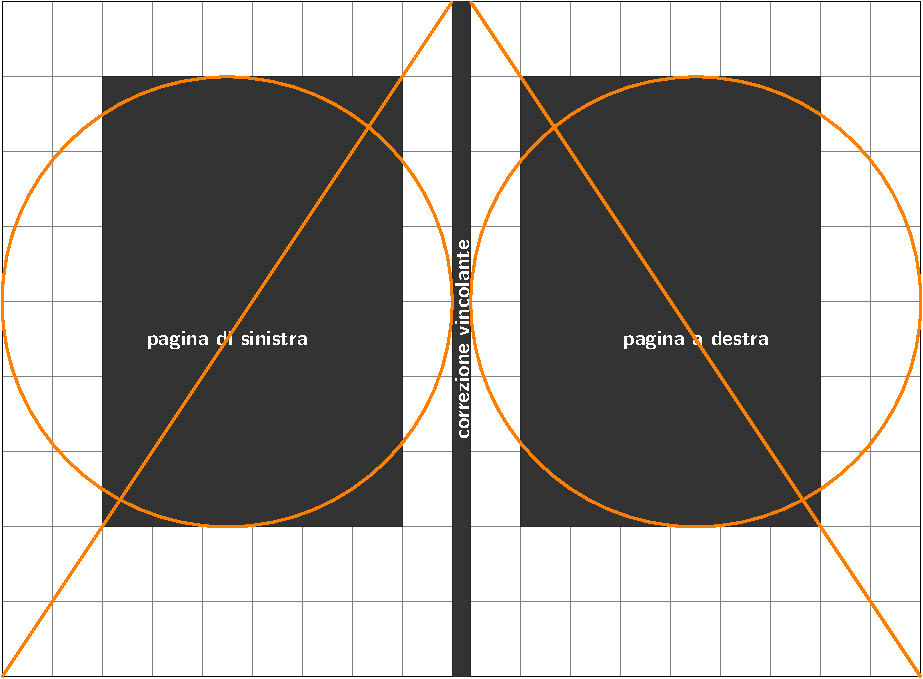
\includegraphics[width=0.9\textwidth]{test-04}
%   \caption{Diagram illustrating page geometry as per the Canons of
%   Page Construction.}
%   \label{fig:canons}
%   \end{figure}
%
%
%    \begin{macrocode}
\newlength\paperwidth@cx
\newlength\paperheight@cx
\newlength\lefttrim
\newlength\bottomtrim
\newlength\bindingcorrection
\setlength\paperwidth@cx{12in}
\setlength\paperheight@cx{18in}
\setlength\bindingcorrection{0.5in}

\cxset{spread xsteps/.store in=\spreadxsteps@cx,
       spread scale/.store in=\spreadscale@cx,
       spread width/.store in=\spreadwidth@cx}
%
%
\cxset{spread xsteps=9,
       spread scale=0.25,
       spread width=0.5\textwidth}% does not work

\tikzset{typearea/.style={color=black!85,fill=black!80,
         font={\sffamily\bfseries}}}
%
%    \end{macrocode}
%
% \begin{macro}{\drawcanons}
%   The macro |\drawcanons| draws a spread, showing all lines and divisions
%   as per classical rules.
%
%    \begin{macrocode}
\def\drawcanons{%
  \begin{tikzpicture}[scale=\spreadscale@cx]
   % draw the two pages
  \draw[xstep=(\paperwidth@cx)/\spreadxsteps@cx,
        ystep=(\paperheight@cx)/\spreadxsteps@cx,color=gray]  (0,0)
    grid (\paperwidth@cx,   \paperheight@cx);
  \draw (0,0) rectangle (\paperwidth@cx,\paperheight@cx);

  \begin{scope}[xshift=\paperwidth@cx+\bindingcorrection]
    \draw[xstep=(\paperwidth@cx)/9,
          ystep=(\paperheight@cx)/9,color=thegray] ++(0,0)
          grid (\paperwidth@cx, \paperheight@cx);
    \draw[color=black] (0,0) rectangle (\paperwidth@cx,\paperheight@cx);
  \end{scope}
%    \end{macrocode}
%
%   Next we draw the binding correction\index{binding correction}. This is drawn as a rectangle. We fill
%   it with the same style shading as the type area.
%
%    \begin{macrocode}
\draw[typearea, draw] (\paperwidth@cx,0)
      rectangle ++(\bindingcorrection, \paperheight@cx);
%    \end{macrocode}
%
%   The typed area blocks are added next.
%
%    \begin{macrocode}
\draw[typearea] (2\paperwidth@cx/\spreadxsteps@cx,
                     2\paperheight@cx/\spreadxsteps@cx)
      rectangle  ++(6/9*\paperwidth@cx,6*\paperheight@cx/\spreadxsteps@cx);

\draw[typearea] (\paperwidth@cx+\paperwidth@cx/9+\bindingcorrection,
     2\paperheight@cx/9) rectangle ++(6\paperwidth@cx/9,6\paperheight@cx/9);

\ifdim\bindingcorrection>0pt
\begin{scope}[typearea,color=white]
\draw node at
      (\paperwidth@cx+0.5\bindingcorrection,
       0.5\paperheight@cx)[rotate=90,inner sep=0pt,outer sep=0pt]
       {\translate{bindingcorrectionname}};
\fi
\node  at
       (0.5\paperwidth@cx,0.5\paperheight@cx){\translate{leftpagename}};
\node  at
      (1.5\paperwidth@cx+\bindingcorrection,
       0.5\paperheight@cx){\translate{rightpagename}};
\end{scope}
%    \end{macrocode}
%   Next we draw the diagonals and the circles. We draw them within
%   a scope to separate the styling from the drafting.
%    \begin{macrocode}
\begin{scope}[color=orange, line width=1pt]
  \draw (0,0)-- (\paperwidth@cx,\paperheight@cx);
  \draw (2\paperwidth@cx+\bindingcorrection,0)--
    ++(-\paperwidth@cx,\paperheight@cx);
%    \end{macrocode}
%
%   The circles are drawn in the same style as the diagonals. We
%   do not provide an option to change this, as it will produce ugly
%   diagrams.
%
%    \begin{macrocode}
\draw (0.5\paperwidth@cx,5\paperheight@cx/9)
       circle (0.5\paperwidth@cx);
\draw [xshift=\paperwidth@cx+\bindingcorrection]
      (0.5\paperwidth@cx,5\paperheight@cx/9)
       circle (0.5\paperwidth@cx);
\end{scope}
\end{tikzpicture}
}
%    \end{macrocode}
% \end{macro}
%
%   \section{Try Layouts}
%
%   The try layouts code, are helper macros to draw dimension lines on a
%   diagram to experiment with different dimensions and layouts.
%   In addition to this some helper commands are incorporated for readabilty.
%
%   \section{Readability}
%
%   In general the width of the typed area should not exceed 45-65 characters.
%   This is language and reader dependent.
%
% \begin{macro}{\alphabet}
%   The macro |\alphabet| returns the twenty six letters of the English
%   language. This is used later on to calculate the length of an
%   alphabet and provide related metrics for the readability of the text.
%
%    \begin{macrocode}
\def\alphabet{%
  \normalfont\selectfont\raggedleft%
   abcdefghijklmnopqrstuvwxyz}
%    \end{macrocode}
% \end{macro}
%
% \begin{macro}{\charactersperline}
%   The macro |charactersperline| typesets the number of characters in
%   a line of text. We use |\pgfmathprintnumber| to format and print
%   the number.
%
%    \begin{macrocode}
\newcommand\charactersperline{%
  \settowidth{\@tempdima}{\alphabet}
  \pgfmathparse{\textwidth/\@tempdima*26}
  \pgfmathprintnumber{\pgfmathresult}
}
%    \end{macrocode}
% \end{macro}
%
% \begin{macro}{\alphabetsperline}
%   Some people are more familiar with the metric alphabets per line
%   rather than characters per line. We provide the macro |\alphabetsperline|.
%
%    \begin{macrocode}
\newcommand\alphabetsperline{%
  \settowidth{\@tempdima}{\alphabet}
  \pgfmathparse{\textwidth/\@tempdima}
  \pgfmathresult
}
%    \end{macrocode}
% \end{macro}
%

% \begin{macro}{\alphabetlength}
%   The macro |\alphabetlength| prints the length of the alphabet.
%
%    \begin{macrocode}
\newcommand\alphabetlength{%
  \settowidth{\alphlength}{\alphabet}
  \pgfmathparse{\alphlength}
  \pgfmathprintnumber{\pgfmathresult}pt
}
%    \end{macrocode}
% \end{macro}
%
% We need to use the fp package to calculate the ratios, as PGF has problems with large
% dimensions or I am making an error
%    \begin{macrocode}
\newcommand\textarearatio{%
    \FPmul{\result}{\strip@pt\textwidth}{\strip@pt\textheight}
    \FPmul{\resulti}{\strip@pt\paperwidth}{\strip@pt\paperheight}
    \FPdiv{\resultii}{\result}{\resulti}
    \pgfmathprintnumber{\resultii}
}

% Calculate the ratio textheight/paperheight
\newcommand\textheightratio{%
    \FPdiv{\result}{\strip@pt\textheight}{\strip@pt\paperheight}
    \FPround{\result}{\result}{2}
    \result
}

% Calculate textheight/paperwidth

\newcommand\textheighttopaperwidth{%
    \pgfmathparse{\textheight/\paperwidth}
    \pgfkeys{/pgf/number format/.cd,fixed,precision=2}
    \pgfmathprintnumber{\pgfmathresult}
}
\newcommand\numbertextlines{%
% baselineskip to be corrected
   \pgfmathparse{(\textheight-\topskip)/(12)-1}\pgfmathresult
}
%    \end{macrocode}
% \begin{macro}{\printreadability}
%    \begin{macrocode}
\def\printreadability{%
\begin{tabular}{lr}
  Characters per line &\charactersperline\\
  Alphabets per line &\alphabetsperline\\
  Alphabet length &\alphabetlength\\
  Baselineskip & \the\baselineskip\\
  Number of text lines &\numbertextlines\\
\end{tabular}}
%    \end{macrocode}
% \end{macro}
%
%   \section{Page Layout Diagrams}
%   This is one of the most important features of the package. Drawing
%   and annotating a page diagram, so that you can view new
%   geometry or use them for notes.
%
%   \subsection{New lengths}
%
%   We need to isolate the current page dimensions from the
%   new trial sizes for the diagram. We redefine new lengths for
%   all parameters with the prefix |try| and the suffix |@cx|.
%
%    \begin{macrocode}
\newlength\trypaperwidth@cx
\newlength\trypaperheight@cx
\newlength\trytextheight@cx
\newlength\tryheadheight@cx
\newlength\tryheadsep@cx
\newlength\tryfootskip@cx
\newlength\trymargintop@cx
\newlength\trymarginbottom@cx
\newlength\trytopmargin@cx
\newlength\trimtop@cx
\setlength\trimtop@cx{0pt}
\newlength\trytextwidth@cx
\newlength\trymarginparwidth@cx
\newlength\trymarginparsep@cx
\newlength\tryleftmargin@cx
\newlength\tryinner@cx
%    \end{macrocode}

%    The stockheight and stockwidth are used when the paper is to be trimmed
%    they default to the dimensions for paper width and paper height,
%    if not specified. The |memoir| class also defines them. If they are
%    defined, we use the values from the class.
%
% \begin{macro}{\stockheight}
% \begin{macro}{\stockwidth}
%    \begin{macrocode}
\@ifundefined{stockheight}{\global\newlength\stockheight}{}
\@ifundefined{stockwidth}{\global\newlength\stockwidth}{}

\ifdim\stockheight=0pt\addtolength\stockheight{\paperheight}\fi
   \addtolength\stockheight{0mm}
\ifdim\stockwidth=0pt\addtolength\stockwidth{\paperwidth}\fi
   \addtolength\stockwidth{0mm}

\newlength\trystockheight@cx
\newlength\trystockwidth@cx
\cxset{try stockwidth/.code=\setlength\trystockwidth@cx{#1},
          try stockheight/.code=\setlength\trystockheight@cx{#1},
          try stock/.code=} % a4paper etc to be developed toninght
\cxset{try stockwidth=\paperwidth}
\cxset{try stockheight=\paperheight}
%    \end{macrocode}
% \end{macro}
% \end{macro}
%   We set all the trims to zero to start with.
%    \begin{macrocode}
%
\newlength\trimtop
\newlength\trimedge
\setlength\lefttrim{5mm}
\setlength\bottomtrim{10pt}
\setlength\trimtop{0pt}
\setlength\trimedge{0pt}
%
%
% set defaults
\setlength\trymargintop@cx{0pt}
\setlength\trymarginparsep@cx{\marginparsep}
\setlength\trymarginparwidth@cx{\marginparwidth}
\setlength\trytextwidth@cx{0pt}
\newlength\trytrimedge@cx
\setlength\trytrimedge@cx{10pt}

\newlength\tryoddsidemargin@cx
\setlength\tryoddsidemargin@cx{\oddsidemargin}
\newlength\tryevensidemargin@cx
\setlength\tryevensidemargin@cx{\evensidemargin}
\newlength\tryinnermargin@cx
%   convenience lengths for drawing the layouts.
\newlength\tryINNER
\newlength\tryTOP

\newlength\margintop

\newcommand\thetop{%
   \pgfmathparse{1in+\topmargin+\headheight+\headsep}
   \pgfmathsetlength{\margintop}{\pgfmathresult}
}
%

\thetop

\newlength\marginbottom
\newcommand\thebottom{%
   \pgfmathparse{\stockheight-(1in+\topmargin+\headheight+\headsep+\textheight)}
    \pgfmathsetlength{\marginbottom}{\pgfmathresult}
  }

\thebottom
%    \end{macrocode}
%
%   We provide keys to set all trial dimensions. These default to the
%   current document, dimensions.
%
%    \begin{macrocode}
\cxset{try textheight/.code=\global\setlength\trytextheight@cx{#1},
       try textheight/.default=\textheight,
       try headheight/.code=\global\setlength\tryheadheight@cx{#1},
       try headheight/.default=\headheight, % TO CHECK
       try headsep/.code=\global\setlength\tryheadsep@cx{#1},
       try headsep/.default=\headsep, %TODO CHECK
       try footskip/.code=\global\setlength\tryfootskip@cx{#1},
       try footskip/.default=\footskip,
       try topmargin/.code=\global\setlength\trytopmargin@cx{#1},
       try topmargin/.default=\topmargin,
}

\cxset{try trimtop/.code=\global\setlength\trimtop@cx{#1},
       try trimtop/.default=\global\setlength\trimtop{0pt},}

% set all the defaults

\cxset{try textheight,
       try headheight,
       try headsep,
       try footskip,
       try topmargin=0pt, % compensate for trim
       try trimtop=10pt}

\setlength\trytopmargin@cx{\topmargin}


\cxset{try textwidth/.code=\global\setlength{\trytextwidth@cx}{#1},
       try trimedge/.code=\global\setlength{\trytrimedge@cx}{#1},
}

\cxset{try textwidth=\textwidth,
       try trimedge=10pt}
%    \end{macrocode}
%
% \begin{macro}{\@trydiagonal}
%   The switch |\@trydiagonal| is used in keys to draw or skip the Page
%   Construction Canon, diagonal line.
%
%    \begin{macrocode}
\newif\if@trydiagonal
\@trydiagonalfalse

\cxset{try diagonal/.is choice,
       try diagonal/true/.code=\@trydiagonaltrue,
       try diagonal/false/.code=\@trydiagonalfalse,
       try diagonal/none/.code=\trydiagonalfalse}

\cxset{try diagonal=false}
%    \end{macrocode}
% \end{macro}
%
% \begin{macro}{\trygrid}
%   The try grid conditional provides a switch to switch the
%   grid on or off. We set it initially to true.
%
%    \begin{macrocode}
\newif\iftrygrid
\trygridfalse

\cxset{try grid/.is choice,
       try grid/true/.code=\trygridtrue,
       try grid/false/.code=\trygridfalse,
       try grid/none/.code=\trygridfalse}

\cxset{try grid=true}
%    \end{macrocode}
% \end{macro}
%
%   \subsection{Allowances for trims}
%
%   Throughout we are focusing on the average LaTeX user than might want
%   to for example use A4 paper and trim down to a different size.
%   We start form the stockwidth and stockheight and we set the
%   paperwidth and paperheight to a smaller size to cater for these trims.
%
%   I call this process trimming in, whereas other packages such as the |crop|
%   increase the paper size to allow for the trims, thus displaying a larger
%   page. The |memoir| class has something similar.
%
% \begin{macro}{\trypaperwidth@cx}
% \begin{macro}{\trypaperheight@cx}
%   We set the length to stocksize-trimedge.
%    \begin{macrocode}
% set the trial paper sizes as per trim sizes
\addtolength\trypaperwidth@cx{\trystockwidth@cx}
\addtolength\trypaperwidth@cx{-\trytrimedge@cx}
\addtolength\trypaperheight@cx{\trystockheight@cx}
\addtolength\trypaperheight@cx{-\trimtop@cx}
\addtolength\trypaperheight@cx{-\bottomtrim}
%    \end{macrocode}
% \end{macro}
% \end{macro}
%
%   \subsubsection{Calculating the Top Margin and Bottom Margin}
%
%   We calculate the top and bottom margins for convenience. Remember that so
%   far we are only dealing with default settings. I the user changes the
%   dimensions, these will have to be recalculated.
%
%    \begin{macrocode}
%\addtolength\trymargintop@cx{1in+\voffset+\trimtop@cx}
%\addtolength\trymargintop@cx{\dimexpr(\tryheadsep@cx+
%   \tryheadheight@cx+\trytopmargin@cx)}
%    \end{macrocode}
%
%    \subsubsection{Adjustments to text height}
%
%    Since we are trimming-in, our paper height will end up being
%    smaller than the stock paper height. One is thus faced with the
%    decision to either make the top and bottom margins smaller to allow
%    for the trimming or to reduce the text height accordingly.
%
%    Most people and publishers are fussy about margins, so perhaps it is
%    better to reduce the text-height. We offer a method to the user
%    to specify preferences later on. In the meantime for the purpose
%    of defaults, we will take all the adjustment at the bottom margin and
%    leave the text-height untouched.
%
% \begin{macro}{\trytextheight@cx}
%   Let |trytextheight@cx| equal to the current document |\textheight|
%   value.
%
%    \begin{macrocode}
\setlength\trytextheight@cx{\textheight}
%    \end{macrocode}
% \end{macro}
%
%    \begin{macrocode}
\setlength\trymarginbottom@cx{%
   \dimexpr(\trystockheight@cx-1in-\trimtop@cx-\trytopmargin@cx
     -\tryheadheight@cx-\tryheadsep@cx-\trytextheight@cx)\relax}


\newlength\stepx
%    \end{macrocode}
%
%   \subsection{Drawing the Trial Layout}
%
%   The trial layout is drawn in a lengthy TikZ picture. If no new
%   dimensions are provided by the user it will default to the values
%   we have set it previously. That is the current layout values.
%
% \begin{macro}{\drawtriallayout}
%   The macro |\drawtriallayout| draws the page diagram. It uses throughout
%   trial dimensions.
%
%    \begin{macrocode}
\tikzset{dim/.style = {color=black,>=latex}}
\def\drawtriallayout{%
%    \end{macrocode}
%
%   We first need to check if we are on an odd or even page and
%   set the geometry accordingly. If the document is one-side we
%   default to drawing everything as an odd-side page.
%
%    \begin{macrocode}
\checkoddpage%
\if@twoside\else\oddpagetrue\fi
\ifoddpage
  \global\setlength\tryinnermargin@cx{\tryoddsidemargin@cx}
  \setlength\tryINNER{\dimexpr(1in+\tryinnermargin@cx+\hoffset)}
 \else
   \global\setlength\tryinnermargin@cx{\tryevensidemargin@cx}
   \setlength\tryINNER{\dimexpr(1in+\tryinnermargin@cx+\hoffset)}
\fi

   \hspace*{-2cm}\begin{tikzpicture}[scale=0.42,font={\scriptsize\rmfamily},line width=.8pt,
       every node={color=black},
       book trim/.style={color=theblue,fill=white},
       dim text/.style={color=black},
       textblock/.style={fill=gray,opacity=0.3}]

\edef\tol{-2.5\baselineskip}
%    \end{macrocode}
%    \begin{macrocode}
%
\def\drawpaperwidthdim{%
    \coordinate (A) at (0,\tol);
    \coordinate (B) at (\trystockwidth@cx -\trytrimedge@cx,\tol);
    \coordinate (C) at (0.5\trystockwidth@cx,\tol);
    \draw [dim, |<->|] (A) -- (B);
    \node at (C) [yshift=0.5\baselineskip)]
    {paper width = \convert@cx{\trypaperwidth@cx} $(W_p)$};}

%  Draw paper width dimension
\def\drawpaperwidthevendim{%
    \coordinate (A) at (0+\trytrimedge@cx,\tol);
    \coordinate (B) at (\trystockwidth@cx,\tol);
    \coordinate (C) at (0.5\trystockwidth@cx,\tol);
    \draw[dim, |<->|] (A) -- (B);
    \node at (C) [yshift=0.5\baselineskip)]
    {paper width = \convert@cx{\trypaperwidth@cx} $(W_p)$};
}
%    \end{macrocode}
%
%   \subsubsection{Draw stock paper}
%   First we draw the stockwidth and stockheight
%
%    \begin{macrocode}
\draw [color=thegray] (0,0) rectangle
           ++(\trystockwidth@cx,\trystockheight@cx);

% draw the paper if trims are defined and no book size given
% the paper width is then defined by the dashed blue line
\ifoddpage
  \draw [book trim]  (0+\lefttrim,\trystockheight@cx-\trimtop@cx)
        rectangle ++(\trystockwidth@cx-\lefttrim-\trytrimedge@cx,
        -\trystockheight@cx+\trimtop@cx+\bottomtrim);
        \drawpaperwidthdim
 \else
  \draw [book trim]  (0+\lefttrim+\trytrimedge@cx,\trystockheight@cx-\trimtop@cx)
        rectangle ++(\trystockwidth@cx-\lefttrim-\trytrimedge@cx,
        -\trystockheight@cx+\trimtop@cx+\bottomtrim);
       \drawpaperwidthevendim
\fi

%    \end{macrocode}
%
%   \subsubsection{Draw grid}
%
%   Unlike the grid on page spreads we provide a conditional to
%   switch it off if necessary. It set to true by default.
%
%   \begin{macrocode}
\pgfmathsetmacro{\gridx}{10}
\iftrygrid
  \ifoddpage
    \draw[xstep=(\trypaperwidth@cx-\lefttrim)/\gridx,
        ystep=\trypaperheight@cx/\gridx,color=thegreen!50,
        line  width=0.4pt,yshift=\bottomtrim,xshift=\lefttrim]
       (0,0) grid (\trypaperwidth@cx-\lefttrim,\trypaperheight@cx);
  \else
    \draw[xstep=(\trypaperwidth@cx)/\gridx,
        ystep=\trypaperheight@cx/\gridx,color=thegreen,
        line width=0.4pt,yshift=\bottomtrim,xshift=\trytrimedge@cx]
        (0,0) grid ++(\trypaperwidth@cx,\trypaperheight@cx);
  \fi
\fi
%    \end{macrocode}
%
%   \subsubsection{Drawing the binding correction}
%   The binding correction is added to the stockheight. It will appear on
%   the opposite site in the even page.
%
%    \begin{macrocode}
\ifoddpage
 \draw (0, \trystockheight@cx + 3mm) -- ++ (0,1cm)
        ++ (\lefttrim,-1cm) -- ++(0,1cm) ++(-1cm-\lefttrim,-0.5cm)[->,>=latex]
        -- ++(0.5cm+\lefttrim,0);
 \draw (0, \trystockheight@cx + 3mm)
        ++ (0,0.5cm) -- ++ (\lefttrim,0)
        ++(1cm,0cm)[|->,>=latex]-- ++(-1cm,0cm)
        node[right] at ++(1cm,0)
        {\translate{bindingcorrectionname}\ \convert@cx{\lefttrim} $(\delta_b)$ };
\fi

% stockwidth dimension lines
\edef\tol{-5\baselineskip}
\coordinate (BD) at (0,\tol);
\coordinate (BD2) at (\stockwidth,-5\baselineskip);
\draw[dim, |<->|] (BD) -- (BD2);
\draw (BD) ++ (0.5\stockwidth,0)
   node [yshift=0.5\baselineskip]
   {stockwidth=\convert@cx{\stockwidth} $(W_s)$} ;

% top dimension at left
\coordinate (H1) at (-5mm,\trystockheight@cx-\trimtop@cx);
\coordinate (H2) at (-5mm,
    \trystockheight@cx-1in-\trimtop@cx-\trytopmargin@cx-
    \tryheadheight@cx-\tryheadsep@cx);
\draw [dim,|<->|] (H1) -- (H2);
\node[left,text width=1.0cm, text centered,dim text] at
   (-5mm,\trystockheight@cx-0.5*\margintop)
   {top\\ \convert@cx{\the\margintop}\\$(h_{t})$};

% bottom dimension at left
\coordinate (H3) at (-5mm,0+\bottomtrim);
\coordinate (H4) at (-5mm,\trymarginbottom@cx);
\draw [dim,|<->|] (H3) -- (H4);
\node[left,text width=1.5cm,text ragged left]
   at (-5mm,0.5*\trymarginbottom@cx)
   {bottom\\ \convert@cx{ \the\trymarginbottom@cx}\\
    $(h_{b})$};

% textheight at left
\draw[dim,<->]  (-5mm, \trymarginbottom@cx)
   -- ++ (0,\trytextheight@cx);
\node[left,text width=1.6cm,text centered,dim text]
   at (-5mm,\trymarginbottom@cx+0.5\trytextheight@cx)
   {\CS{textheight} \convert@cx{\trytextheight@cx}\\
   $(h_x)$ };

%    \end{macrocode}

%   \subsubsection{Book height}
%
%   Book sizes are specified by the size of the final trimmed sizes. for
%   most users there is no need to worry about trims and binding
%   corrections, however we provide these for consistency and for books
%   that are perhaps to be sent to an on-line bureau for printing.

%    \begin{macrocode}
\draw [dim,|<->|] (-4.7cm,\bottomtrim) --
  (-4.7cm,0.5\trystockheight@cx-0.5\trimtop@cx)
  node[left,text width=1.2cm,text centered,dim text]
  {\translate{bookheightname}\\ \convert@cx{\trypaperheight@cx}} --
  (-4.7cm,\trystockheight@cx-0.5\trimtop@cx) ;
%    \end{macrocode}

%   \subsubsection{Draw the edge trim}
%   The paper is always assumed to be trimmed at top bottom and the edge
%   margin. We first draw the edge trim and its dimension.
%
%    \begin{macrocode}
\ifdim\trytrimedge@cx>0pt
 \ifoddpage
   \coordinate (D) at (\trystockwidth@cx-4\trytrimedge@cx,
                       0.10\trytextheight@cx);
   \coordinate (E) at (\trystockwidth@cx,0.10\trytextheight@cx);
   \draw [dim,->|] (D) -- ++(3\trytrimedge@cx,0);
   \draw [dim,|<-|] (E) -- ++(3\trytrimedge@cx,0)
     node at ++(0,0) [right,text width=2cm,dim text]
     {\translate{trimedgename}\
     \convert@cx{\the\trytrimedge@cx}
     $(\Delta_e)$};
 \else
  \coordinate (D1) at (0, \trystockheight@cx+ 5mm);
  \coordinate (E1) at ++ (\trytrimedge@cx,\stockheight+\trimtop@cx);
  \draw (D1) -- ++ (0, 10mm)  ++(\trytrimedge@cx,0) -- ++(0,-10mm) ;
 \fi
\fi
%    \end{macrocode}
%   \subsubsection{The top trim}
%   The top trim is drawn next. As it is very small normally we try
%   not to crowd the label and the dimension lines. We will only show it
%   if it has a value.
%
%    \begin{macrocode}

%\ifdim\trimtop>0pt
  \coordinate (F) at (0.9\trystockwidth@cx,\trystockheight@cx-\trimtop@cx-8mm);
  \coordinate (G) at (0.9\trystockwidth@cx,\trystockheight@cx-\trimtop@cx);
  \coordinate (H) at (0.9\trystockwidth@cx,\trystockheight@cx);
  \draw (F)[dim,->|,>=latex] -- (G);
  \draw (H) -- ++ (0,8mm) -- ++ (5mm,0)[|<-|,>=latex]
          node [text width=2cm, right] at ++ (0,3pt) {\translate{trimtopname}\
          \\ \convert@cx{\the\trimtop@cx} $(\Delta_t)$};
%\fi
%    \end{macrocode}
%
%   \subsubsection{Driver offsets}
%
%   Next we draw the driver offsets. The lines are drawn at the left side
%   of the paper both for even and for odd paper. Of course they are meaningless
%   if the printer is going to print them on an A3 paper for example, and then
%   the paper is trimmed.
%
%    \begin{macrocode}
   \draw[fill=olive] (1in,\trystockheight@cx-1in) circle (1.5mm);
   \draw[dashed,color=olive] (1in,0) -- (1in,\trystockheight@cx);
   \draw[dashed,color=olive] (0in,\trystockheight@cx-1in)-- ++ (\trystockwidth@cx,0);
   \draw [dim,|<->|](0,0.3cm)-- (1in,0.3cm) node at (0.5in,0.6)[dim text] {\translate{oneinchname}};
%    \end{macrocode}
%
%	Draw the inner margin. We use innermargin which has already been set
%	to either oddsidemargin or evensidemargin
%    \begin{macrocode}

% 	Draw left = 1in + innermargin
\setlength\tryleftmargin@cx{\dimexpr(1in+\innermargin)}
\draw [dim,|<->|] (0in,1.9cm) -- (1in+\innermargin,1.9cm)
node at (0.6in,3.2cm)[text width=1in,dim text,text centered]
{$(w_i)$\\ \convert@cx{\tryleftmargin@cx}\\inner margin};

 \draw (1in,1.2cm)[|<->|] -- ++(\innermargin,0) node[right,dim text]
 {\innermarginname\   \convert@cx{\the\innermargin} $(\Delta_i)$};


%   add topmargin dimension

\setlength{\@tempdimc}{\dimexpr(1in-\trimtop@cx+\trytopmargin@cx)\relax}
\coordinate (S1) at (\trystockwidth@cx+3ex,\trystockheight@cx-\trimtop@cx);
\draw [dim,|<->|] (S1)
      -- ++ (0,-\@tempdimc-\trimtop@cx)
      node [right, dim text, text width=3.5cm] at
      ++(2ex,0.5\@tempdimc) {\convert@cx{\@tempdimc} $(\delta_t)$
\\ \textbackslash topmargin \convert@cx{\trytopmargin@cx}};
%    \end{macrocode}
%
%   \subsubsection{Draw the running head}
%   The running head is drawn measuring from the
%   top of the page.
%    \begin{macrocode}
\pgfmathsetlength{\@tempdimb}{\trystockheight@cx-
                    \trimtop@cx-1in-\trytopmargin@cx}

 \draw[textblock] (\tryINNER, \@tempdimb)
         rectangle ++ (\trytextwidth@cx,-\tryheadheight@cx);

%  add headheight dimension
\draw [dim,-|,>=stealth] (\trystockwidth@cx+3ex, \@tempdimb)
        -- ++(0,-\tryheadheight@cx) node [right,dim text] at
        ++(2ex,0.3\tryheadheight@cx)
        {\CS{headheight} \convert@cx{\the\tryheadheight@cx} $(h_{h,h})$};
%
%%   add headsep dimension
\draw [dim,|-,] (\trystockwidth@cx+3ex,
      \@tempdimb-\tryheadheight@cx-\tryheadsep@cx)
       -- ++(0,\tryheadsep@cx) node [right, dim text] at
       ++(2ex,-0.8\tryheadsep@cx){\CS{headsep}
       \convert@cx{\the\tryheadsep@cx} $(h_{h,s})$};
%    \end{macrocode}

%   \subsubsection{Type area}
%
%   Next we add the type area and its dimension.
%
%    \begin{macrocode}
\coordinate (J) at (\tryINNER,
     \@tempdimb-\tryheadsep@cx-\tryheadheight@cx);
\draw[textblock] (J) rectangle ++ (\trytextwidth@cx,-\trytextheight@cx);
\draw[dim,<->|,dim text] (\tryINNER,0.75\trytextheight@cx)
  -- ++(\trytextwidth@cx, 0)
  node at ++(-0.5\trytextwidth@cx,0.8\baselineskip){\labelit@cx{\textwidth}};

%   add textheight dimension
\draw [dim,<->] (\trystockwidth@cx+3ex,
       \@tempdimb-\tryheadsep@cx-\tryheadheight@cx) --
       ++(0,-\trytextheight@cx) node [right, dim text, text width=2.5cm]
       at ++(2ex,0.5\trytextheight@cx)
       {\CS{textheight}\\ \convert@cx{\the\trytextheight@cx}$(h_x)$};
%    \end{macrocode}
%
%   \subsubsection{Footer}
%   Add the footer and its dimension.
%    \begin{macrocode}
\coordinate (I) at (\tryINNER,
          \@tempdimb-\tryheadsep@cx-
          \tryheadheight@cx-\trytextheight@cx-\tryfootskip@cx);
\draw[textblock] (I) rectangle ++ (\trytextwidth@cx,\tryheadheight@cx);
\draw [dim,|<->|,>=stealth] (\trystockwidth@cx+3ex,\@tempdimb-\tryheadsep@cx-
    \tryheadheight@cx-\trytextheight@cx) --
    ++(0,-\tryfootskip@cx) node [right, dim text] at
    ++(2ex,0.5\tryfootskip@cx){%
    \labelit@cx{\tryfootskip@cx}$(h_f)$};
%
%
% marginpar
\def\leftmarginpar{%
   \draw [textblock] (\tryINNER+\trytextwidth@cx+\trymarginparsep@cx,
         \@tempdimb-\tryheadsep@cx-\tryheadheight@cx) rectangle ++(\trymarginparwidth@cx,-\trytextheight@cx);
 \draw [dim,|<->|] (\tryINNER+\trytextwidth@cx+\trymarginparsep@cx
   +\trymarginparwidth@cx,0.75\trytextheight@cx)
   -- ++ (-\trymarginparwidth@cx,0) node at
   ++(0.5\trymarginparwidth@cx,0.7\baselineskip)
   {marginparwidth} node at ++(0.5\trymarginparwidth@cx,-\baselineskip)
   {\convert@cx{\the\trymarginparwidth@cx} $(w_{m,w})$};

%	Draw the marginsep dimension above
 \draw [dim,|-|] (\tryINNER+\trytextwidth@cx,0.85\trytextheight@cx)
          -- ++ (\trymarginparsep@cx,0)
         node[right,dim text,text width=2cm,text centered] at
         ++(-3ex,12pt) {marginparsep\\ \convert@cx{\trymarginparsep@cx} $(w_{m,s})$ };
}
%
\def\rightmarginpar{%
 \draw [textblock] (\tryINNER-\trymarginparsep@cx,
   \@tempdimb-\tryheadsep@cx-\tryheadheight@cx)
   rectangle ++(-\trymarginparwidth@cx,-\trytextheight@cx);
 \draw [dim,|<->|] (\tryINNER-\trymarginparsep@cx-\trymarginparwidth@cx,
     0.75\trytextheight@cx) -- ++ (\trymarginparwidth@cx,0) node at
     ++(-0.5\trymarginparwidth@cx,0.5\baselineskip) {marginparwidth.} node at
     ++(-0.5\marginparwidth,-\baselineskip){\convert@cx{\the\marginparwidth}};
 }
%
%
\drawmarginparstrue
\ifdrawmarginpars
  \ifoddpage
    \leftmarginpar
   \else
     \rightmarginpar
  \fi
\fi
%    \end{macrocode}
%
%   \subsubsection{Page Construction Canon Diagonal Lines}
%
%   I the conditional |@trydiagonal| is set to |true| draw the diagonal lines.
%   At |false| or |none| skip.
%
%    \begin{macrocode}
\if@trydiagonal
  \ifoddpage
     \draw [color=blue!30](\trystockwidth@cx-\trytrimedge@cx,\bottomtrim)
       -- (\lefttrim, \trystockheight@cx-\trimtop@cx);
  \else
    \draw [color=blue!30] (\trytrimedge@cx,0)
    -- (\paperwidth,\paperheight-\trimtop@cx);
  \fi
\fi
\end{tikzpicture}
}

%    \end{macrocode}
% \end{macro}

%	\section{Lists}
%	List diagrams are developed using the techniques we have used so far for the pages.
%	We define layouts to visualize them.
%     \begin{figure}
%	   \centering
%        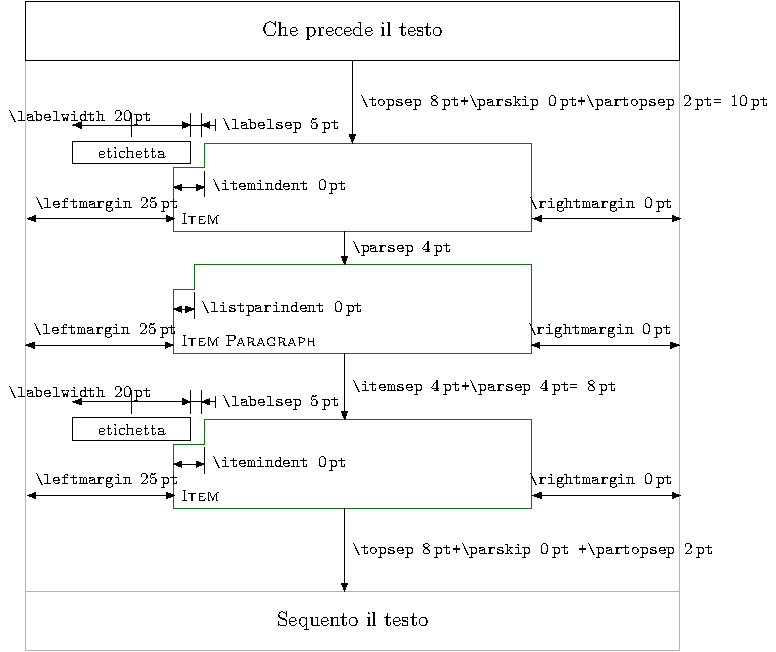
\includegraphics[width=0.8\textwidth]{test-03}
%	   \caption{List diagram, showing LaTeX geometry definitions.}
%      \label{fig:listdiagram}
%     \end{figure}
%
% \begin{macro}{\drawlist}
%	The macro |\drawlist| draws an outline of an enumerated or any type of list
%	illustrating the main parameters affecting its layout. It is based on ideas presented
%	originally in the |layouts| package and a sample is shown in
%   figure~\ref{fig:listdiagram}
%    \begin{macrocode}
\newlength\tempa@cx
\newlength\tempb@cx
\newlength\tempc@cx
\newlength\listdiagramheight
\newlength\listdiagramwidth

\def\drawlistdiagram{%
  \begin{tikzpicture}[scale=0.5,dim/.style={font={\footnotesize}},
                                           block/.style={color=thegreen}]	
  \pgfmathsetmacro{\yscale}{8}
  \pgfmathsetlength{\tempa@cx}{\yscale*(\topsep+\parskip+\partopsep)}
  \pgfmathsetlength{\tempb@cx}{\yscale*(\itemsep+\parsep)}
  \pgfmathsetlength{\tempc@cx}{\yscale*(\parsep)}
  \pgfmathsetlength{\listdiagramheight}{13cm+2*\tempa@cx+\tempb@cx+\tempc@cx}
  \pgfmathsetlength{\listdiagramwidth}{\textwidth+10cm}
%    \end{macrocode}
%	We first draw a block to reprsesent some text and the block on a page.
%    \begin{macrocode}
\draw[color=thegray!60] (0,0) rectangle (\listdiagramwidth,\listdiagramheight);
\draw[color=thegray!60] (0,0) rectangle (\listdiagramwidth, 2cm);
\draw (0,\listdiagramheight) rectangle (\listdiagramwidth,\listdiagramheight-2cm)
         node at ++ (-0.5\listdiagramwidth,1cm){\translate{precedingtextname}};
\node at (0.5\listdiagramwidth,1cm) {\translate{followingtextname}};
%    \end{macrocode}
%	Next we are going to draw the item shape. First we draw the rectangle
%	with the indentation.
% \begin{macro}{\putlistblock@cx}
%    \begin{macrocode}
\def\putlistblock@cx##1##2{%
  \coordinate (A) at (##1,##2);
  \coordinate (B) at (##1-40pt,##2-20pt);
  \draw[block]   (A) -- ++ (\textwidth,0pt)
                     -- ++ (0, 3cm)
                     -- ++ (-\textwidth+ 30pt,0)
                     -- ++ (0, -24pt)
                     -- ++ (-30pt,0)
                     -- ++ (0,-3cm+24pt);
 % dra wthe label rectangle
  \draw[block,color=black]  (B) ++ (-2cm, 3cm) rectangle ++ (4cm, 22pt )
      node[dim] at ++(-2cm,-11pt) {\translate{labelname}};
  % draw dimension lines
  \draw  (B) ++ (0, 3cm+26pt) -- ++ (0,0.8cm) ++ (2cm,-0.8cm)--++(0,0.8cm) ++ (10pt,-0.8cm)
          --++ (0,0.8cm); %labelsep
% draw arrows
  \settowidth\@tempdima{labelwidth}
  \draw[dim] [<->,>=latex] (B) ++ (-2cm, 3cm+26pt)++(0,0.4cm)-- ++(4cm,0)
    node[dim] at ++ (- 2cm-\@tempdima-50pt,8pt)
    {\labelit@cx{\labelwidth}};

  \draw[dim] (B)  ++ (0, 3cm+26pt+0.4cm) -- ++ (2cm+10pt,0)
                   ++ (0.5cm,0)--++(-0.5cm,0)[|->,>=latex]
                   node[right] at ++(0.45cm,0) {\labelit@cx{\labelsep}};
%	draw itemsep

  \draw[<->,>=latex] (A)++(0,1.5cm) -- ++(30pt,0) ;
  \draw (A)++(30pt,1.20cm )--++ (0pt,1.8cm-27pt) node at ++(0,0)[below right]
  {\labelit@cx{\itemindent}}; % draw dimline
    \node[dim] (A) at (##1,##2)[above right] {\textsc{Item}};

%    draw leftmargin and right margin

\draw[<->,>=latex] (A) ++ (-24pt,0pt) -- ++(-5cm,0pt)
         node at ++(0,0)[above right] {\labelit@cx{\leftmargin}};
\draw[<->,>=latex] (A) ++ (-24pt+\textwidth,0pt) -- ++(5cm,0pt)
        node at ++(0,0)[above left] {\labelit@cx{\rightmargin}};
}
%
%
\def\putlistparblock@cx##1##2{%
  \coordinate (A) at (##1,##2);
  \coordinate (B) at (##1-40pt,##2-20pt);
  \draw[block]   (A) -- ++ (\textwidth,0pt)
                     -- ++ (0, 3cm)
                     -- ++ (-\textwidth+ 20pt,0)
                     -- ++ (0, -24pt)
                     -- ++ (-20pt,0)
                     -- ++ (0,-3cm+24pt);

  \draw[<->,>=latex] (A)++(0,1.5cm) -- ++(20pt,0) ;
  \draw (A)++(20pt,1.20cm )--++ (0pt,1.8cm-27pt) node at ++(0,0)[below right]
        {\labelit@cx{\listparindent}};

   \draw[<->,>=latex] (A) ++ (-0pt,8pt) -- ++(-5cm,0pt)
         node at ++(0,0)[above right] {\labelit@cx{\leftmargin}};
   \draw[<->,>=latex] (A) ++ (0pt+\textwidth,8pt) -- ++(5cm,0pt)
        node at ++(0,0)[above left] { \labelit@cx{\rightmargin}};

   \node[dim] (A) at (##1,##2)[above right] {\textsc{Item Paragraph}};
}

%
%	We start by drawing the blocks. We draw three blocks, the first and last show items, whereas
%	the middle one shows a paragraph within an item.
%	Since values for list parameters are small, we scale everything up.
%     |\tempa@cx = scaled topsep + parskskip + partopsep|
%     |\tempb@cx = scaled itemsep + parsep|
%
%	 \end{macrocode}
%	 \begin{macrocode}
\putlistblock@cx{5cm}{2cm+\tempa@cx} % 8cm
\draw [<-,>=latex] (0.5\paperwidth, 2cm)-
            -++(0,\tempa@cx) node at ++(0,-0.5\tempa@cx) [right]
            {\labelit@cx{\topsep}+\labelit@cx{\parskip} +\labelit@cx{\partopsep}};

%	second block
\putlistparblock@cx{5cm}{2cm+\tempa@cx+3cm+\tempb@cx}
\draw [->,>=latex] (0.5\paperwidth, 2cm+\tempa@cx+3cm+\tempb@cx)--++(0,-\tempb@cx)
      node at ++(0,0.5\tempb@cx) [right]
      {\labelit@cx{\itemsep}+\labelit@cx{\parsep}=
          \pgfmathparse{\itemsep+\parsep}\convert@cx{\pgfmathresult}};

%% third block
\putlistblock@cx{5cm}{2cm+\tempa@cx+6cm+\tempb@cx +\tempc@cx}
\draw [->,>=latex] (0.5\paperwidth,2cm+\tempa@cx+6cm+\tempb@cx +\tempc@cx )
      --++(0,-\tempc@cx)
      node at ++(0,0.5\tempc@cx) [right] {\labelit@cx{\parsep}};

% add finally the top arrow
\draw [->,>=latex] (0.5\listdiagramwidth, \listdiagramheight-2cm)--++(0,-\tempa@cx)
     node at ++(0,0.5\tempa@cx) [right]
{\labelit@cx{\topsep}+\labelit@cx{\parskip}+\labelit@cx{\partopsep}=
     \pgfmathparse{\topsep+\parskip+\partopsep}\convert@cx{\pgfmathresult}};

%
%    \end{macrocode}
% \end{macro}

%    \begin{macrocode}
\end{tikzpicture}
}
%    \end{macrocode}
% \end{macro}
%
%

%   \subsection{Tabulating List values}
% \begin{macro}{\printlistvalues}
%   The command |\printlistvalues| produces a short table showing the
%   list parameters and their values (see Table~\ref{tbl:listvalues} for
%   an example).
%
%   \begin{table}[htbp]
%   \begin{quote}
%   \item ~~\par
%   \centering
%   \cxset{geometry units=pc}
%   \printlistvalues
%   \end{quote}
%   \caption{Tabulation of LaTeX list values, for the \textit{quotation}
%    environment.}
%   \label{tbl:listvalues}
%   \end{table}
%
%    \begin{macrocode}
\def\printlistvalues{%
  \begin{tabular}{lr}
    \toprule
    Parameter    & Value\\
    \midrule
    leftmargin   & \convert@cx{\the\leftmargin}\\
    rightmargin  & \convert@cx{\the\rightmargin}\\
    itemindent   & \convert@cx{\itemindent}\\
    labelwidth   & \convert@cx{\labelwidth}\\
    labelsep     & \convert@cx{\labelsep}\\
    listparindent& \convert@cx{\listparindent}\\
    topsep       & \convert@cx{\topsep}\\
    partopsep    & \convert@cx{\partopsep}\\
    parsep       & \convert@cx{\parsep}\\
    itemsep      & \convert@cx{\itemsep}\\
    \bottomrule
    \end{tabular}
}
%    \end{macrocode}
% \end{macro}
%
%   \section{Draw a Font box}
%   We provide a command that can draw a box and font dimensions. We
%   will use TikZ for drafting and styling. We also provide the macro
%   |\printfontparams| to print font parameters. This will produce a table
%   as shown in Table~\ref{tbl:fontdetails} and Table~\ref{tbl:fontdimensions}.
%
%   \begin{table}[htbp]
%   \centering
%   \printfontparams
%   \caption{Font details for the current document font.}
%   \label{tbl:fontdetails}
%   \end{table}
%
%
%   \begin{table}[htbp]
%   \centering
%   \printfontdimensions
%   \caption{Font dimension details for the current document font.}
%   \label{tbl:fontdimensions}
%   \end{table}
%
%   \cxset{geometry units=pc}
%
%   To draw a fontbox, we use
%   \medskip
%
%   \drawfontbox{fjord}
%   \medskip
%
%   This draws \drawfontframe{Q}\drawfontframe{werty}.
%
%
% \begin{macro}{\printfontparams}
%    \begin{macrocode}
\newcommand{\printfontparams}{%
  \begin{tabular}{lc}
     \toprule
     Parameter     & Value\\
     \midrule
     Font encoding & \f@encoding\\
     font family   & \f@family\\
     font series   & \f@series\\
     font shape    & \f@shape\\
     font size     & \f@size\\
     baselineskp   & \f@baselineskip\\
     \bottomrule
     \end{tabular}
 }
%    \end{macrocode}
% \end{macro}
%
% \begin{macro}{\printfontdimensions}
%    \begin{macrocode}
\newcommand{\printfontdimensions}{%
  \begin{tabular}{lc}
  \toprule
  Parameter     & Value\\
  \midrule
    fontdimen1 (slant per point)  is & \the\fontdimen1\font\\
    fontdimen2 (interword space)     & \the\fontdimen2\font\\
    fontdimen3 (interword stretch)          & \the\fontdimen3\font\\
    fontdimen4 (interword shrink)          & \the\fontdimen4\font\\
    fontdimen5 (x-height)  & \the\fontdimen5\font\\
    fontdimen6 (quad width)& \the\fontdimen6\font\\
    fontdimen7 (extra space) & \the\fontdimen7\font\\
  \bottomrule
  \end{tabular}
 }
%    \end{macrocode}
% \end{macro}
%
% \begin{macro}{\drawfontframe}
% \begin{macro}{\drawfontbox}
%   The macro |\drawfontbox|\marg{text} draws text in a box and annotates it with dimensions.
%   A very similar macro is defined in Peter Wilson's \package{layouts}. I thought
%   with TikZ it can be drawn more easily than the tens of lines of |put| in
%   the original macros.
%
%   We define some new length to hold temporary values for the fontbox
%   dimensions, although PGF provides its own methods.
%
%    \begin{macrocode}
\newlength\xheight@cx
\newlength\xwidth@cx
\newlength\xdepth@cx
\newlength\xtotal@cx
\newsavebox{\fontbox}
%    \end{macrocode}
%
%   We set a number of keys to enable styling the box.
%
%    \begin{macrocode}
\cxset{fontbox font/.store in=\fontboxfont@cx,
       fontbox line color/.store in=\fontboxlinecolor@cx,
       fontbox label font/.store in=\fontboxlabelfont@cx}

%   Set reasonable defaults
%
\cxset{fontbox font={\itshape\Huge},
       fontbox line color=thered,
       fontbox label font={\upshape\footnotesize}}
%    \end{macrocode}
%
%   Define a macro to draw a tight frame around text. This can be
%   used for inline text and hence we use |\tikz| to define it. We align it
%   using |baseline=(X.base)|.
%   See (\href{http://tex.stackexchange.com/questions/58281%
%   /how-to-align-a-series-of-tikz-pictures-at-the-baseline}
%   {How to align a series of tikz pictures at the baseline.})
%
%   See also \href{http://tex.stackexchange.com/questions/
%   58283/tikz-how-to-determine-
%   the-vector-between-two-co-ordinates#comment122802_58283}{how to determine the
%   vector between two co-ordinates.}
%    \begin{macrocode}
\newcommand\drawfontframe[1]{%
  \tikz[baseline=(X.base), font=\fontboxlabelfont@cx]{%
    \node[rectangle,draw,inner sep=0pt,outer sep=0pt,
          color=\fontboxlinecolor@cx] (X)[black]{#1};
    \draw[\fontboxlinecolor@cx, line width=0.4pt] (X.text)
      circle(0.4pt)[fill=red] -- (X.base east);}
}
%
\def\drawfontbox#1{%
   {\itshape\fontboxfont@cx
   \savebox{\fontbox}{#1}
   \pgfmathsetlength{\xheight@cx}{\ht\fontbox}
   \pgfmathsetlength{\xwidth@cx}{\wd\fontbox}
   \pgfmathsetlength{\xdepth@cx}{\dp\fontbox}
   \pgfmathsetlength{\xtotal@cx}{\xdepth@cx+\xheight@cx}
  \begin{tikzpicture}[scale=1,label/.style={font={\fontboxlabelfont@cx}}]
    \node[rectangle,draw,inner sep=0pt,outer sep=0pt] (X){#1};
    \draw[red, line width=0.4pt,label] (X.text)  circle(1pt)[fill=red] -- (X.base east);
    \draw[|<->|,>=latex] ([yshift=5pt] X.north west)
       --([yshift=5pt] X.north east) node [label,above=-5pt,midway]{width = \convert@cx{\xwidth@cx}};
%    \end{macrocode}
%
%   We next draw the x-height of the text
%    \begin{macrocode}
    % draw the xheight
    \draw[|<->|,>=latex,label]([xshift=-5pt]X.base west)
          --([xshift=-5pt] X.north west)
          node [left,midway,label] {x-height=\convert@cx{\xheight@cx}};
%   draw depth
    \draw[-|,>=latex,label]([xshift=-5pt]X.base west)
          --([xshift=-5pt] X.south west)
          node [left,midway,label] {depth=\convert@cx{\xdepth@cx}};
    \draw[<-,>=latex]([xshift=-5pt]X.south west)
          --++(0,-8pt);
%   draw total height
%
\draw[|<->|,>=latex,label]([xshift=5pt]X.north east)
          --([xshift=5pt] X.south east)
          node [right,midway] {height=\convert@cx{\xtotal@cx}};

  \end{tikzpicture}}
}
%    \end{macrocode}
% \end{macro}
% \end{macro}
%
%
% \subsection{Sundry}%
% Here are assorted macro definitions.
% \begin{macro}{\lineloop}
% \begin{macro}{\linefoot}
% The (document-level) command \cmd\lineloop\ sets numbered lines until the
% specified count is reached.
% The command \cmd\linefoot\ sets a single, automatically numbered line,
% but with a footnote (with the specified label);
% it automatically increments the line counter.
% These commands are typically used to construct test documents.
%
% Because the counter is globally advanced and never reset, successive
% calls to \cmd\lineloop\ should have an argument ever larger.
% The formatted output will have each line labeled with its ordinal number.
%    \begin{macrocode}
\newcounter{linecount}
\def\loop@line#1#2{%
 \par
 \hb@xt@\hsize{%
  \global\advance#1\@ne
  \edef\@tempa{\@ifnum{100>#1}{0}{}\@ifnum{10>#1}{0}{}\number#1}%
  \@tempa\edef\@tempa{\special{line:\@tempa}}\@tempa
  \vrule depth2.5\p@#2\leaders\hrule\hfil
 }%
}%
\def\lineloop#1{%
 \loopwhile{\loop@line\c@linecount{}\@ifnum{#1>\c@linecount}}%
}%
\def\linefoot#1{%
 \loop@line\c@linecount{%
  \footnote{%
   #1\special{foot:#1}\vrule depth2.5\p@\leaders\hrule\hfill
  }%
 }%
}%
%    \end{macrocode}
% \end{macro}
% \end{macro}
%


% \iffalse
%</package>
% \fi
%
%    \section{Minimal Working Examples (MWE)}
%
%	We generate a number of examples to illustrate usage and to
%	test the code. The first example \texttt{test-01.tex}, uses the
%	standard book class. It also uses a number of pictures
%	to illustrate float parameter placement.
%
% \iffalse
%<*test-01>
% \fi
%   \begin{macrocode}
\documentclass[twoside,10pt]{book}
\usepackage{tikz,changepage,fancyhdr,amsmath,booktabs}
\usepgflibrary{arrows}
\usepackage{lipsum}
\usepackage[german]{babel}
\usepackage[german]{xlayouts}
\renewcommand{\topfraction}{.6}
\renewcommand{\bottomfraction}{.8}
\renewcommand{\textfraction}{.04}
\renewcommand{\floatpagefraction}{.9} % have a high one don't encourage it
\renewcommand{\dbltopfraction}{.5}
\renewcommand{\dblfloatpagefraction}{.8}
\setcounter{topnumber}{9}
\setcounter{bottomnumber}{9}
\setcounter{totalnumber}{2}
\setcounter{dbltopnumber}{1}
\pagestyle{grid}
\begin{document}
\section{Introduction}
\thispagestyle{grid}
\begin{figure}[b]
\ifbotfloat{\figureparamsbot}{%
 \iftopfloat{\figureparamstop}{}}

\centering
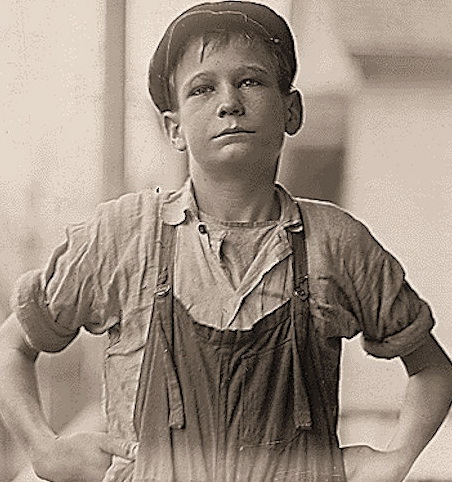
\includegraphics[height=0.9\columnwidth]{./images/hine04-x}
\caption{Example image to demonstrate top fraction.}
\end{figure}
\lipsum[1]

\lipsum[1]

This has been drawn using TikZ\footnote{A kleine program.}\footnote{Another footnote.}.
\lipsum[1-2]
\begin{figure}[t]
 \caption{Example image to demonstrate top.}
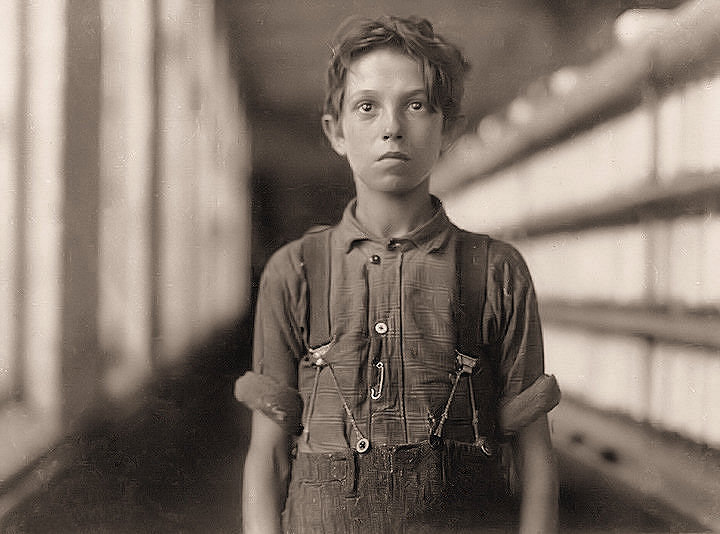
\includegraphics[width=\columnwidth]{./images/hine02}%
  \iftopfloat{\figureparamstop}{}
\end{figure}
\begin{figure}[tpb]
\centering
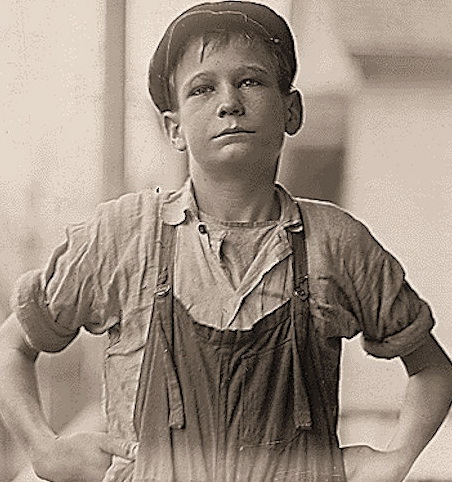
\includegraphics[height=\columnwidth]{./images/hine04-x}
\caption{Example image to demonstrate top fraction.}
\end{figure}

\begin{figure}[tpb]
\centering
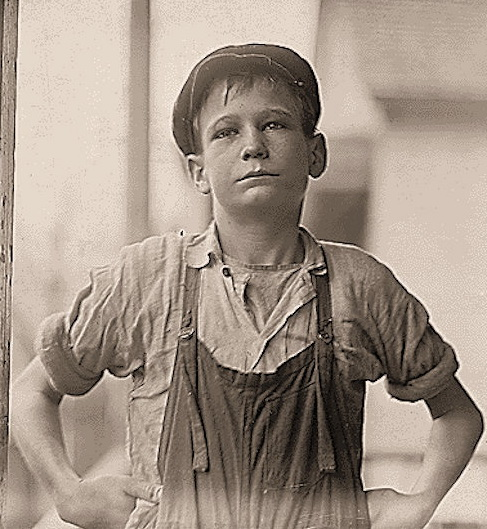
\includegraphics[width=\columnwidth]{./images/hine04-xx}
\caption{Example image to demonstrate top fraction.}
\end{figure}
\lipsum
\clearpage
\onecolumn
%   draws the spread

\drawcanons

\printreadability
\pagestyle{plain}
\newpage
% draws a trial layout
\drawtriallayout
\newpage
\drawtriallayout
\newpage
\drawlistdiagram
\printlistvalues
\end{document}
%    \end{macrocode}
%
% \iffalse
%</test-01>
% \fi
%
%
%
%
%
%
%<*test-02>
%    \begin{macrocode}
%%
%% File: test-02.tex
%% Tests xlayout for scrbook class.
%% 26/05/2012
%%
%%
\documentclass[twoside,10pt]{scrbook}
\usepackage{tikz,changepage,fancyhdr,amsmath}
\usepgflibrary{arrows}
\usepackage{lipsum}
\uspackage[german]{babel}
\usepackage[german]{xlayouts}
\renewcommand{\topfraction}{.6}
\renewcommand{\bottomfraction}{.8}
\renewcommand{\textfraction}{.04}
\renewcommand{\floatpagefraction}{.9} % have a high one don't encourage it
\renewcommand{\dbltopfraction}{.5}
\renewcommand{\dblfloatpagefraction}{.8}
\setcounter{topnumber}{9}
\setcounter{bottomnumber}{9}
\setcounter{totalnumber}{2}
\setcounter{dbltopnumber}{1}
\pagestyle{grid}
\begin{document}
\section{Introduction}
\thispagestyle{grid}
\begin{figure}[b]
\ifbotfloat{\figureparamsbot}{%
 \iftopfloat{\figureparamstop}{}}

\centering
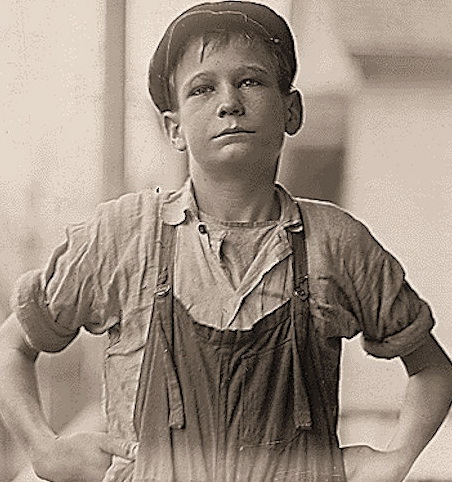
\includegraphics[height=0.9\columnwidth]{./images/hine04-x}
\caption{Example image to demonstrate top fraction.}
\end{figure}
\lipsum[1]

\lipsum[1]

This has been drawn using TikZ\footnote{A kleine program.}\footnote{Another footnote.}.
\lipsum[1-2]
\begin{figure}[t]
 \caption{Example image to demonstrate top.}
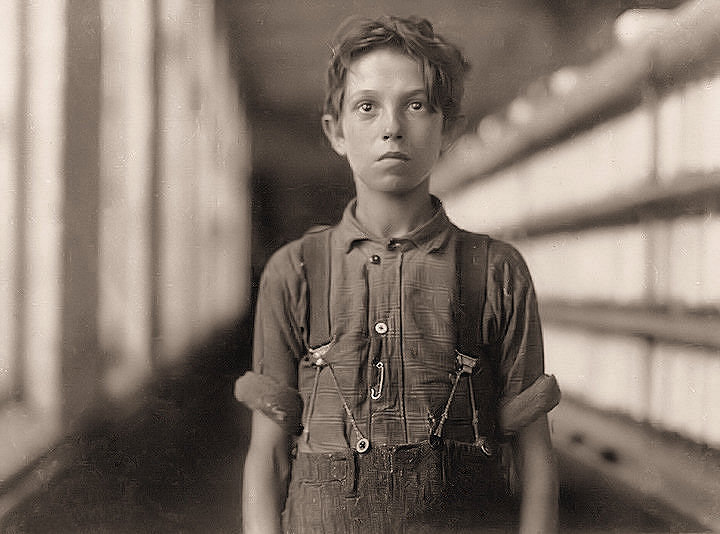
\includegraphics[width=\columnwidth]{./images/hine02}%
  \iftopfloat{\figureparamstop}{}
\end{figure}
\begin{figure}[tpb]
\centering
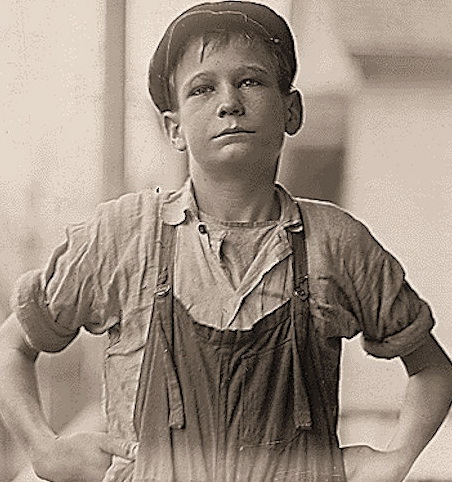
\includegraphics[height=\columnwidth]{./images/hine04-x}
\caption{Example image to demonstrate top fraction.}
\end{figure}

\begin{figure}[tpb]
\centering
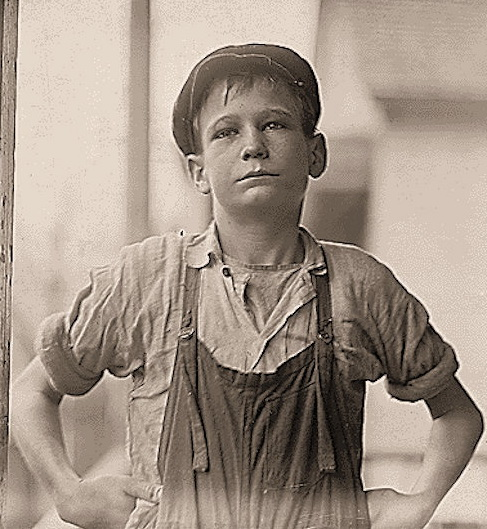
\includegraphics[width=\columnwidth]{./images/hine04-xx}
\caption{Example image to demonstrate top fraction.}
\end{figure}
\lipsum
\clearpage
\onecolumn
%   draws the spread
\drawcanons

\printreadability
\pagestyle{plain}
\newpage
% draws a trial layout
\drawtriallayout
\newpage
\drawtriallayout
\end{document}
%
%    \end{macrocode}
%</test-02>
%
%	\subsection{List standalone diagram MWE}
%
%<*test-03>
%    \begin{macrocode}
%%	This file is generated automatically by xlayouts.dtx.
%%	It produces a standalone diagram for lists.
%%	
\documentclass{standalone}
\usepackage[italian]{babel}
\usepackage[italian]{xlayouts}
\begin{document}
\drawlistdiagram
\end{document}
%    \end{macrocode}
%</test-03>
%
%<*test-04>
%    \begin{macrocode}
%%	This file is generated automatically by xlayouts.dtx.
%%	It produces a standalone diagram for lists.
%%	
\documentclass{standalone}
\usepackage[italian]{babel}
\usepackage[italian]{xlayouts}
\begin{document}
\drawcanons
\end{document}
%    \end{macrocode}
%</test-04>
%<*test-05>
%    \begin{macrocode}
%%	This file is generated automatically by xlayouts.dtx.
%%	It produces a two page spread and shows the dimensions.
%%	
\documentclass[twoside]{book}
\usepackage[left=80pt,right=80pt,top=0.75in]{geometry}
\usepackage[final]{graphicx}
\usepackage{lipsum}
\usepackage{xlayouts}
\makeatletter
\providecommand{\cleartoevenpage}[1][\@empty]{%
 \clearpage%
 \ifodd\c@page\null#1\clearpage\fi}
\makeatother
\pagestyle{grid}
\begin{document}
\mainmatter
\null\newpage
\pgfpagesuselayout{2 on 1}[a3paper,landscape,border shrink=0mm]
%% first page
\cleartoevenpage
\checkoddpage%
{\parindent0pt
\vbox to 120pt{\lipsum[1]}%
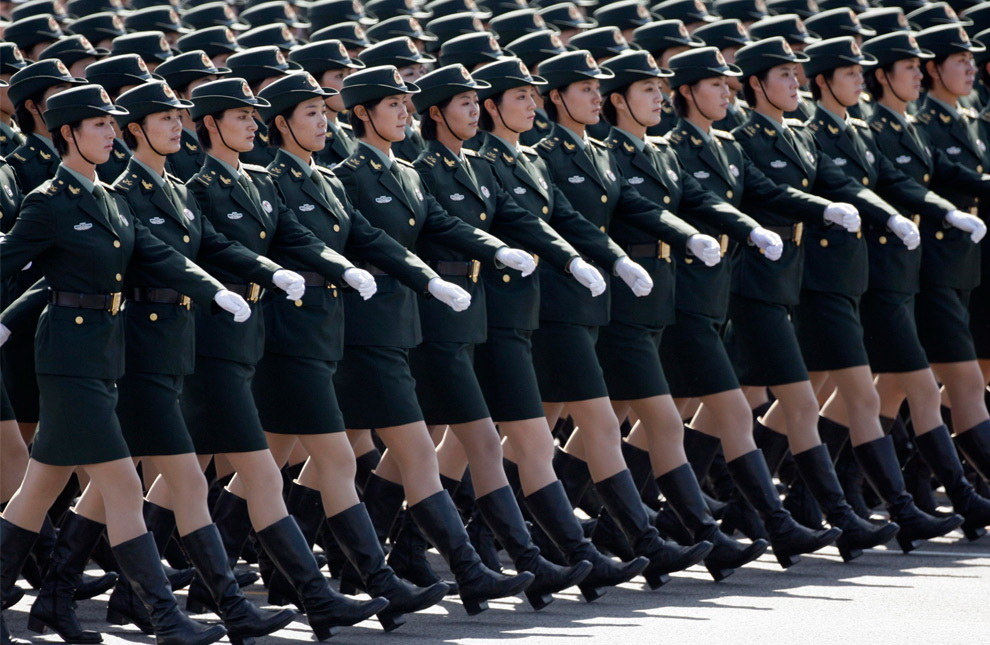
\includegraphics[height=0.78\textheight]{china-05}}

%%secondpage
{\parindent0pt
\vbox to 120pt{\lipsum[1]}%
\hspace*{\dimexpr(-2in-\textwidth-2\evensidemargin)}
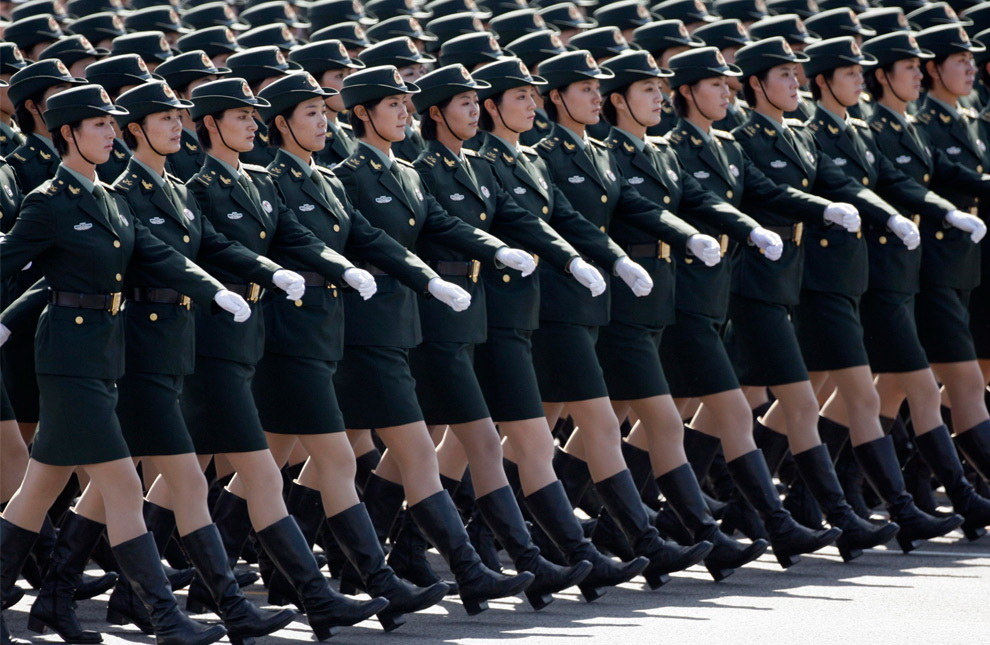
\includegraphics[height=0.78\textheight]{china-05}}
\hspace{2.8em}\parbox[b]{0.571\textwidth}{%
\section*{\hfill CHINA PARADE \hfill\hfill}
\lipsum[1-3]}
\end{document}
%    \end{macrocode}
%</test-05>



%
%	\section{Dictionaries}
%<*english>
%%   This file is generated automatically
%%   and it contains translation strings for the English language.
%%   it is saved in a file pages-German.dict according to
%%   the conventions of the translator package.
%%
%    \begin{macrocode}
\ProvidesDictionary{pages-English}{English}
\providetranslation{headername}{header}
\providetranslation{bodyname}{body}
\providetranslation{footername}{footer}
\providetranslation{marginnotename}{margin note}
\providetranslation{oneinchname}{one inch}
\providetranslation{notshownname}{not shown}
\providetranslation{drivermarginname}{driver margin}
\providetranslation{leftpagename}{left page}
\providetranslation{rightpagename}{right page}
\providetranslation{bindingcorrectionname}{binding correction}
\providetranslation{bookheightname}{book height}
\providetranslation{trimedgename}{trim edge}
\providetranslation{trimtopname}{top trim}
\providetranslation{trimbottomname}{bottom trim}
\providetranslation{precedingtextname}{Preceding Text}
\providetranslation{followingtextname}{Following Text}
\providetranslation{labelname}{label}
%    \end{macrocode}
%
%</english>
%
%
%<*german>
%%   This file is generated automatically
%%   and it contains translation strings for the German language.
%%   it is saved in a file pages-German.dict according to
%%   the conventions of the translator package.
%%
%    \begin{macrocode}
\ProvidesDictionary{pages-German}{German}
\providetranslation{headername}{Kopfzeile}
\providetranslation{bodyname}{Haupttext}
\providetranslation{footername}{Fu{\ss}zeile}
\providetranslation{marginnotename}{Rand-\\ notizen}
\providetranslation{oneinchname}{ein Zoll}
\providetranslation{notshownname}{ohne Abbildung}
\providetranslation{drivermarginname}{Fahrer-Marge}
\providetranslation{leftpagename}{Linke Seite}
\providetranslation{rightpagename}{Rechte Seite}
\providetranslation{bindingcorrectionname}{Bindekorrektur}
\providetranslation{bookheightname}{Buch H\"ohe}
\providetranslation{trimedgename}{Schnittkante}
\providetranslation{trimtopname}{Trim-Top}
\providetranslation{trimbottomname}{trim Unten}
\providetranslation{precedingtextname}{Che precede il testo}
\providetranslation{followingtextname}{Sequento il testo}
\providetranslation{labelname}{label}
%    \end{macrocode}
%
%</german>
%
%
%<*italian>
%%   This file is generated automatically
%%   and it contains translation strings for the German language.
%%   it is saved in a file pages-German.dict according to
%%   the conventions of the translator package.
%%
%    \begin{macrocode}
\ProvidesDictionary{pages-Italian}{Italian}
\providetranslation{headername}{testatina}
\providetranslation{bodyname}{corpo}
\providetranslation{footername}{piedino}
\providetranslation{marginnotename}{note marginale}
\providetranslation{oneinchname}{un piedino}
\providetranslation{notshownname}{non mostrato}
\providetranslation{drivermarginname}{conducente del margine}
\providetranslation{leftpagename}{pagina di sinistra}
\providetranslation{rightpagename}{pagina a destra}
\providetranslation{bindingcorrectionname}{correzione vincolante}
\providetranslation{bookheightname}{libro di altezza}
\providetranslation{trimedgename}{cimosse}
\providetranslation{trimtopname}{top asseto}
\providetranslation{trimbottomname}{fondo assetto}
\providetranslation{precedingtextname}{Che precede il testo}
\providetranslation{followingtextname}{Sequento il testo}
\providetranslation{labelname}{etichetta}
%    \end{macrocode}
%
%</italian>
%
%<*dutch>
%%   This file is generated automatically
%%   and it contains translation strings for the Dutch language.
%%   it is saved in a file pages-German.dict according to
%%   the conventions of the translator package.
%%
%    \begin{macrocode}
\ProvidesDictionary{pages-Dutch}{Dutch}
\providetranslation{headername}{kopregel}
\providetranslation{bodyname}{broodtekst}
\providetranslation{footername}{voetregel}
\providetranslation{marginnotename}{marge notities}
\providetranslation{oneinchname}{een inch}
\providetranslation{notshownname}{niet getoond}
\providetranslation{drivermarginname}{bestuurder marge}
\providetranslation{leftpagename}{linkerpagina}
\providetranslation{rightpagename}{juiste pagina}
\providetranslation{bindingcorrectionname}{binding correctie}
\providetranslation{bookheightname}{book hoekte}
\providetranslation{trimedgename}{snijrand}
\providetranslation{trimtopname}{Trim top}
\providetranslation{trimbottomname}{Trim onderkant}
%    \end{macrocode}
%
%</dutch>
%
%<*french>
%%   This file is generated automatically
%%   and it contains translation strings for the Dutch language.
%%   it is saved in a file pages-German.dict according to
%%   the conventions of the translator package.
%%
%    \begin{macrocode}
\ProvidesDictionary{pages-French}{French}
\providetranslation{headername}{kopregel}
\providetranslation{bodyname}{broodtekst}
\providetranslation{footername}{voetregel}
\providetranslation{marginnotename}{marge notities}
\providetranslation{oneinchname}{een inch}
\providetranslation{notshownname}{niet getoond}
\providetranslation{drivermarginname}{bestuurder marge}
\providetranslation{leftpagename}{linkerpagina}
\providetranslation{rightpagename}{juiste pagina}
\providetranslation{bindingcorrectionname}{binding correctie}
\providetranslation{bookheightname}{book hoekte}
\providetranslation{trimedgename}{snijrand}
\providetranslation{trimtopname}{Trim top}
\providetranslation{trimbottomname}{Trim onderkant}
%    \end{macrocode}
%
%</french>

%<*spanish>
%%   This file is generated automatically
%%   and it contains translation strings for the Dutch language.
%%   it is saved in a file pages-German.dict according to
%%   the conventions of the translator package.
%%
%    \begin{macrocode}
\ProvidesDictionary{pages-French}{French}
\providetranslation{headername}{kopregel}
\providetranslation{bodyname}{broodtekst}
\providetranslation{footername}{voetregel}
\providetranslation{marginnotename}{marge notities}
\providetranslation{oneinchname}{een inch}
\providetranslation{notshownname}{niet getoond}
\providetranslation{drivermarginname}{bestuurder marge}
\providetranslation{leftpagename}{linkerpagina}
\providetranslation{rightpagename}{juiste pagina}
\providetranslation{bindingcorrectionname}{binding correctie}
\providetranslation{bookheightname}{book hoekte}
\providetranslation{trimedgename}{snijrand}
\providetranslation{trimtopname}{Trim top}
\providetranslation{trimbottomname}{Trim onderkant}
%    \end{macrocode}
%
%</spanish>

% The end of the configuration file code
%
% \bibliographystyle{alpha}
% \begingroup
% \raggedright
% \begin{thebibliography}{GMSN94A}
%
%
%    \bibitem[ABH90]{bk:Impatient}
%      Paul W.~Abrahams, Karl Berry and Kathryn A.~Hargreaves.
%      \newblock \emph{TeX{} for the Impatient}.
%      \newblock
%       Addison-Wesley, Reading, Massachusetts, 1990.
%      \newblock (Available from CTAN in \texttt{info/impatient})
%
% \bibitem[Ars01a]{TITLEREF}
% Donald Arseneau.
% \newblock \emph{\Lpack{Titleref} package (version 3.1)}.
% \newblock April 2001.
% \newblock (Available from CTN as
%            \texttt{macros/latex/contrib/misc/titleref.sty})
%
% \bibitem[Ars01b]{CHAPTERBIB}
% Donald Arseneau.
% \newblock \emph{\Lpack{Chapterbib} package (version 1.9)}.
% \newblock September 2001.
% \newblock (Available from CTN as
%            \texttt{macros/latex/contrib/misc/chapterbib.sty})
%
% \bibitem[Ars03]{FRAMED}
% Donald Arseneau.
% \newblock \emph{\Lpack{Framed} package (version 0.8a)}.
% \newblock July 2003.
% \newblock (Available from CTAN as
%            \texttt{macros/latex/contrib/misc/framed.sty})
%
% \bibitem[Ars05]{PLACEINS}
% Donald Arseneau.
% \newblock \emph{\Lpack{Placeins} package (version 2.2)}.
% \newblock May 2005.
% \newblock (Available from CTN as
%            \texttt{macros/latex/contrib/placeins/placeins.sty})
%
%
% \bibitem[ArWi00]{IFMTARG}
% Donald Arseneau and Peter Wilson.
% \newblock \emph{The ifmtarg package}.
% \newblock March, 2000.
% \newblock (Available from CTAN in
%            \texttt{/macros/latex/contrib/misc})
%
%
%  \bibitem[Car94]{DELARRAY}
%  David Carlisle.
%  \newblock \emph{The \Lpack{delarray} package}.
%  \newblock March 1994.
%  \newblock (Available from CTAN in
%             \texttt{/macros/latex/required/tools})
%
%
% \bibitem[Car98a]{ENUMERATE}
% David Carlisle.
% \newblock \emph{The enumerate package}.
% \newblock August, 1998.
% \newblock (Available from CTAN in
%            \texttt{/macros/latex/required/tools})
%
% \bibitem[Car98b]{REMRESET}
% David Carlisle.
% \newblock \emph{The remreset package}.
% \newblock August, 1998.
% \newblock (Available from CTAN in
%            \texttt{/macros/latex/contrib/carlisle})
%
%  \bibitem[Car99]{TABULARX}
%  David Carlisle.
%  \newblock \emph{The \Lpack{tabularx} package}.
%  \newblock January 1999.
%  \newblock (Available from CTAN in
%             \texttt{/macros/latex/required/tools})
%
%  \bibitem[Car01]{DCOLUMN}
%  David Carlisle.
%  \newblock \emph{The \Lpack{dcolumn} package}.
%  \newblock May 2001.
%  \newblock (Available from CTAN in
%             \texttt{/macros/latex/required/tools})
%
% \bibitem[Coc02]{SUBFIGURE}
% Steven Douglas Cochran.
% \newblock \emph{The subfigure package}.
% \newblock March, 2002.
% \newblock (Available from CTAN in
%            \texttt{/macros/latex/contrib/subfigure})
%
% \bibitem[Dal99]{NATBIB}
% Patrick W. Daly.
% \newblock \emph{Natural Sciences Citations and References}.
% \newblock May, 1999.
% \newblock (Available from CTAN in
%            \texttt{/macros/latex/contrib/natbib})
%
% \bibitem[Dow00]{PATCHCMD}
% Michael J. Downes
% \newblock \emph{The patchcmd package}.
% \newblock July 2000.
% \newblock (Available from CTAN in
%            \texttt{/macros/latex/contrib/patchcmd})
%
% \bibitem[Fai98]{MOREVERB}
% Robin Fairbairns.
% \newblock \emph{The moreverb package}.
% \newblock December, 1998.
% \newblock (Available from CTAN in
%            \texttt{/macros/latex/contrib/moreverb})
%
% \bibitem[Fai03]{FOOTMISC}
% Robin Fairbairns.
% \newblock \emph{\Lpack{footmisc} --- a portmanteau package for
%            customising footnotes in LaTeX}.
% \newblock February 2003.
% \newblock (Available from CTAN in
%            \texttt{macros/latex/contrib/footmisc})
%
%
%    \bibitem[Fea03]{BOOKTABS}
%      Simon Fear.
%      \newblock \emph{Publication quality tables in \LaTeX}.
%       \newblock March, 2003.
%      \newblock (Available from CTAN in
%                 \texttt{macros/latex/contrib/booktabs})
%
% \bibitem[Fra00]{CROP}
% Melchior Franz.
% \newblock \emph{The crop package}.
% \newblock February, 2000.
% \newblock (Available from CTAN in
%            \texttt{/macros/latex/contrib/crop})
%
%
% \bibitem[GMS94]{GOOSSENS94}
% Michel Goossens, Frank Mittelbach, and Alexander Samarin.
% \newblock {\em The LaTeX Companion}.
% \newblock Addison-Wesley Publishing Company, 1994.
%
%
%
%  \bibitem[Knu84]{bk:knuth}
%       Donald E. Knuth.
%  \newblock  \emph{The \TeX{}book}.
%  \newblock
%       Addison-Wesley, Reading, Massachusetts, 1984.
%
%
% \bibitem[KWG]{TUFTE}
% Bil Kleb, Bill Wood, and Kevin Godby.
% \newblock \emph{Tufte LaTeX}.
% \newblock December 2009.
% \newblock (Available from CTAN in \texttt{macros/latex/contrib/tufte-latex/})
%
%    \bibitem[Lam94]{bk:lamport}
%       Leslie Lamport.
%       \newblock  \emph{\LaTeX\ --- A Document Preparation System}.
%       \newblock
%       Addison-Wesley, Reading, Massachusetts, 1994.
%
% \bibitem[LMB99]{CLASSES}
% Leslie Lamport, Frank Mittelbach and Johannes Braams.
% \newblock \emph{Standard Document Classes for LaTeX version 2e}.
% \newblock September, 1999.
% \newblock (Available from CTAN as
%            \texttt{/macros/latex/base/classes.dtx})
%
%  \bibitem[MC98]{ARRAY}
%  Frank Mittelbach and David Carlisle.
%  \newblock \emph{A new implementation of LaTeX's tabular and array
%                  environment}
%  \newblock May 1998.
%  \newblock (Available from CTAN in
%             \texttt{/macros/latex/required/tools})
%
% \bibitem[Oos96]{FANCYHDR}
% Piet van Oostrum.
% \newblock \emph{Page layout in LaTeX}.
% \newblock June, 1996.
% \newblock (Available from CTAN in
%            \texttt{/macros/latex/contrib/fancyhdr})
%
%
% \bibitem[Rah01]{NAMEREF}
% Sebastian Rahtz.
% \newblock \emph{Section name references in LaTeX}.
% \newblock January 2001.
% \newblock (Available from CTAN in
%            \texttt{/macros/latex/contrib/hyperref})
%
% \bibitem[Rah02]{HYPERREF}
% Sebastian Rahtz.
% \newblock \emph{Hypertext marks in LaTeX}.
% \newblock March 2002.
% \newblock (Available from CTAN in
%            \texttt{/macros/latex/contrib/hyperref})
%
%
% \bibitem[Sch98]{EVERYSHI}
% Martin Schr\"{o}der.
% \newblock \emph{The everyshi package}.
% \newblock August, 1998.
% \newblock (Available from CTAN in
%            \texttt{/macros/latex/contrib/ms})
%
% \bibitem[SRR01]{VERBATIM}
% Rainer Sch\"{o}pf, Bernd Raichle and Chris Rowley.
% \newblock \emph{A new implementation of LaTeX's verbatim and verbatim*
%                 environments}.
% \newblock March, 2001.
% \newblock (Available from CTAN in
%            \texttt{/macros/latex/required/tools})
%
% \bibitem[Wil99]{TOCVSEC2}
% Peter Wilson.
% \newblock \emph{The tocvsec2 package}.
% \newblock January, 1999.
% \newblock (Available from CTAN in
%            \texttt{/macros/latex/contrib/tocvsec2})
%
% \bibitem[Wil00a]{EPIGRAPH}
% Peter Wilson.
% \newblock \emph{The epigraph package}.
% \newblock February, 2000.
% \newblock (Available from CTAN in
%            \texttt{/macros/latex/contrib/epigraph})
%
% \bibitem[Wil00b]{ISOCLASS}
% Peter Wilson.
% \newblock \emph{LaTeX files for typesetting ISO standards}.
% \newblock February, 2000.
% \newblock (Available from CTAN in
%            \texttt{/macros/latex/contrib/isostds/iso})
%
% \bibitem[Wil00c]{NEXTPAGE}
% Peter Wilson.
% \newblock \emph{The nextpage package}.
% \newblock February, 2000.
% \newblock (Available from CTAN in
%            \texttt{/macros/latex/contrib/misc})
%
% \bibitem[Wil00d]{NEEDSPACE}
% Peter Wilson.
% \newblock \emph{The needspace package}.
% \newblock March, 2000.
% \newblock (Available from CTAN in
%            \texttt{/macros/latex/contrib/misc})
%
% \bibitem[Wil01a]{ABSTRACT}
% Peter Wilson.
% \newblock \emph{The abstract package}.
% \newblock February, 2001.
% \newblock (Available from CTAN in
%            \texttt{/macros/latex/contrib/abstract})
%
% \bibitem[Wil01b]{CHNGPAGE}
% Peter Wilson.
% \newblock \emph{The chngpage package}.
% \newblock February, 2001.
% \newblock (Available from CTAN in
%            \texttt{/macros/latex/contrib/misc})
%
% \bibitem[Wil01c]{APPENDIX}
% Peter Wilson.
% \newblock \emph{The appendix package}.
% \newblock March, 2001.
% \newblock (Available from CTAN in
%            \texttt{/macros/latex/contrib/appendix})
%
% \bibitem[Wil01d]{CCAPTION}
% Peter Wilson.
% \newblock \emph{The ccaption package}.
% \newblock March, 2001.
% \newblock (Available from CTAN in
%            \texttt{/macros/latex/contrib/ccaption})
%
% \bibitem[Wil01e]{CHNGCNTR}
% Peter Wilson.
% \newblock \emph{The chngcntr package}.
% \newblock March, 2001.
% \newblock (Available from CTAN in
%            \texttt{/macros/latex/contrib/misc})
%
% \bibitem[Wil01f]{HANGING}
% Peter Wilson.
% \newblock \emph{The hanging package}.
% \newblock March, 2001.
% \newblock (Available from CTAN in
%            \texttt{/macros/latex/contrib/hanging})
%
% \bibitem[Wil01g]{TITLING}
% Peter Wilson.
% \newblock \emph{The titling package}.
% \newblock March, 2001.
% \newblock (Available from CTAN in
%            \texttt{/macros/latex/contrib/titling})
%
% \bibitem[Wil01h]{TOCBIBIND}
% Peter Wilson.
% \newblock \emph{The tocbibind package}.
% \newblock April, 2001.
% \newblock (Available from CTAN in
%            \texttt{/macros/latex/contrib/tocbibind})
%
% \bibitem[Wil01i]{TOCLOFT}
% Peter Wilson.
% \newblock \emph{The tocloft package}.
% \newblock April, 2001.
% \newblock (Available from CTAN in
%            \texttt{/macros/latex/contrib/tocloft})
%
% \bibitem[Wil01j]{VERSE}
% Peter Wilson.
% \newblock \emph{Typesetting simple verse with LaTeX}.
% \newblock August, 2001.
% \newblock (Available from CTAN in
%            \texttt{/macros/latex/contrib/verse})
%
%
% \bibitem[Wil03]{LEDMAC}
% Peter Wilson.
% \newblock \emph{\Lpack{ledmac}: A presumptuous attempt to port EDMAC and
%                 TABMAC to LaTeX}.
% \newblock August 2003.
% \newblock (Available from CTAN in
%            \texttt{macros/latex/contrib/ledmac})
%
% \bibitem[Wil07]{GLISTER07}
% Peter Wilson.
% \newblock `Glisterings' \emph{TUGboat}, 28(2):229--232,
% \newblock 2007.
%
% \bibitem[Wil08]{GLISTER08}
% Peter Wilson.
% \newblock `Glisterings' \emph{TUGboat}, 29(2):324--327,
% \newblock 2008.
%
%
%
%
%
% \end{thebibliography}
% \endgroup
% \PrintChanges
% \PrintIndex
% \Finale
\endinput
